% soapff-gui：構造ファイルから，SOAP の電荷を使った ClayFF の LAMMPS 入力を自動で作る．コンパイル: tectonic main.tex
\documentclass[a4paper,11pt]{article}
\usepackage[margin=22mm]{geometry}
\usepackage{xeCJK}
\setCJKmainfont{Hiragino Mincho ProN}
\setCJKsansfont{Hiragino Kaku Gothic ProN}
\xeCJKDeclareCharClass{CJK}{"2460->"2473}
\usepackage{amsmath,amssymb}
\usepackage{graphicx}
\usepackage{booktabs}
\usepackage{caption}
\usepackage{hyperref}
\captionsetup{font=small,labelfont=bf}
\renewcommand{\figurename}{図}
\renewcommand{\tablename}{表}
\renewcommand{\refname}{参考文献}
\renewcommand{\abstractname}{概要}
\newcommand{\e}{\,e}
\newcommand{\TBD}{\textbf{[未]}}

\title{SOAP 記述子と原子電荷の一対一の対応による ClayFF 力場の自動生成：\\Na モンモリロナイトと鉱物の結晶での検証，拡散係数と白雲母の力学物性の比較}
\author{Haruto Kono$^{1,2}$, Atsuki Hiraguchi$^{2}$, Masahiko Okumura$^{2}$\\[4pt]
{\small $^{1}$ Department of Earth Science, Graduate School of Science, Tohoku University, Sendai, Japan}\\
{\small $^{2}$ Center for Computational Science \& e-Systems, Japan Atomic Energy Agency, Kashiwa, Chiba, Japan}}
\date{2026年10月（草稿）}

\begin{document}
\maketitle

\begin{abstract}
ClayFF の原子電荷は原子のまわりの局所環境で決まるので，局所環境を表す SOAP 記述子と一対一に対応するはずである．
本稿では，その対応から古典 MD の入力を自動で作るツールを開発し，うまく働くかと，得られる物性が先行研究と合うかを確かめた．
力場は，ClayFF の原論文の表のとおりの ClayFF と，柔軟な SPC 水である．
Na モンモリロナイトの初期構造（2{,}502 原子）では，水と Na$^+$ を含めた全原子で，SOAP がいちばん似た別の原子の電荷は自分と同じだった．
この構造と，石英，アルバイト，ブルーサイト，パイロフィライト，白雲母（2M$_1$，1M），金雲母，Cs 雲母（nanpingite），カオリナイト，リザーダイト，タルクの 12 のバルクの結晶の，全原子の SOAP ベクトルと電荷と型の表（ライブラリ，13 構造，5{,}878 原子）を作ると，すべての原子で一対一の対応が成り立った（$l_{\max}=3$--5）．
元素と座標と箱だけの構造ファイルを渡すと，各原子にライブラリでいちばん似た原子の電荷と型をそのまま与え，型から結合と角度を決めて，LAMMPS の入力一式を書き出す．
これを，ウィンドウで構造ファイルを選んで実行するだけで LAMMPS と解析まで回る GUI ソフトウェア soapff-gui として実装した．
入力ファイルは，エネルギー最小化と 10\,ps の NVT による緩和のあとに，本計算の NVT または NPT を行う．
Na モンモリロナイトの初期構造からは，水が粘土に重なっていても，全原子の電荷と型がライブラリと一致する力場が作られた．
ライブラリと大きさの違う超格子の 12 の結晶（216--720 原子）と，そのうち層状ケイ酸塩 8 つの 300\,K の MD のあとの構造でも，全原子の電荷と型が結合のつながりから決めた ClayFF の型と一致した．
生成した入力は，最小化と緩和を経て，Na モンモリロナイトと 12 の結晶のどの系でも，NVT と NPT まで安定に回った．
さらに，生成した Na モンモリロナイトの力場で 300，330，366\,K の面内の拡散係数を求め，同じ ClayFF と柔軟な SPC 水を用いた Greathouse ら\cite{greathouse2016}の値と比べた．
水の O は 11.7--32.5，Na$^+$ は 4.3--15.3（$10^{-10}$\,m$^2$/s）で，Greathouse らの値の 0.75--0.99 倍，活性化エネルギーは水の O で $14.1\pm1.1$，Na$^+$ で $17.8\pm3.9$\,kJ/mol（Greathouse ら 15.2，16.5\,kJ/mol）だった．
soapff-gui の「＋ 物性」で生成した入力による白雲母 2M$_1$ の 0\,K の弾性定数と 300\,K の引張・せん断の応力--ひずみ曲線は，同じ ClayFF による Teich-McGoldrick ら\cite{teich2012}，DelRio ら\cite{delrio2026}の値とおおむね一致し（引張強度 x，y で 13--15\,GPa，z で 3.5\,GPa），面内の弾性定数を実験より 30--50\,\% 大きく出すという ClayFF の性質も同じだった．
\end{abstract}

\section{はじめに}
粘土鉱物の古典 MD で広く用いられる ClayFF\cite{cygan2004,cygan2021}は，原子を型に分け，型ごとに決まった電荷と Lennard-Jones（LJ）パラメータを与える．
型は局所的な配位で決まる．たとえば八面体シートで Al の代わりに Mg が入ると，その Mg に結合した架橋 O は obos（$-1.1808$\e），結合した OH の O は ohs（$-1.0808$\e）になり，通常の ob（$-1.05$\e），oh（$-0.95$\e）と区別される．
エッジの OH の変角項\cite{pouvreau2017}や結合価数によるエッジの電荷\cite{lammers2017}，物性に合わせた INTERFACE FF\cite{heinz2013}など，型の考え方は拡張されてきたが，いずれも原子ごとに型を決め，水やイオンと合わせて入力ファイルを作る作業が要る．

型が局所的な配位で決まるなら，原子のまわりの配置を表す記述子から型と電荷を決められるはずである．
原子の局所環境を数値のベクトルで表す記述子は，機械学習ポテンシャル\cite{behler2007,bartok2010}とともに発展し，SOAP\cite{bartok2013}はその代表である\cite{willatt2019,musil2021,langer2022}．
SOAP の類似度は構造の比較にも用いられ\cite{de2016}，局所環境から原子電荷を予測する機械学習も報告されている\cite{kancharlapalli2021,raza2020}．

本稿では，次のことを行う．
(i) Na モンモリロナイトの 2 水和層の系を例に，粘土の原子だけでなく水と Na$^+$ も SOAP の対象とし，すべての原子で SOAP と電荷が一対一に対応するか（SOAP がいちばん似た別の原子の電荷が自分と同じか）を確かめる．
(ii) この対応を表（ライブラリ）として保存し，構造ファイルを渡すだけで，SOAP で決めた電荷と型を使った ClayFF の LAMMPS 入力を作り，最小化，緩和，本計算の MD，解析までを行う GUI ソフトウェア soapff-gui を開発する．
Na モンモリロナイトの系で，生成した力場がライブラリのラベルと一致するか，そのまま MD が回るかを確かめる．
(iii) ClayFF の型で表せる石英，アルバイト，ブルーサイト，パイロフィライトと，雲母，カオリン，蛇紋石，タルクの層状ケイ酸塩の結晶を同じライブラリに加え，ライブラリと大きさの違う結晶と MD で乱れた結晶でも，構造ファイルだけから正しい型と電荷が付くかを確かめる．
(iv) 生成した力場で求めた Na モンモリロナイトの層間の水と Na$^+$ の拡散係数とその温度依存性を，同じ ClayFF と SPC 水による先行研究\cite{greathouse2016}と比べる．
(v) soapff-gui が生成する力学物性の計算（弾性定数，引張，せん断）で白雲母を計算し，同じ ClayFF による先行研究\cite{teich2012,delrio2026}と実験\cite{vaughan1986}と比べる．

\section{方法}
\subsection{系}
系は，Mg 置換モンモリロナイトの 2 層と，層間の Na$^+$ 30 個，水 344 分子（2 水和層）からなる（2{,}502 原子，30.96 $\times$ 26.90 $\times$ 25.55\,\AA，図\ref{fig:system}）．
粘土の層電荷は $0.83$\e{} / O$_{20}$(OH)$_4$（八面体の Mg 置換，Na$_{0.83}$[Al$_{3.17}$Mg$_{0.83}$]Si$_8$O$_{20}$(OH)$_4$），水は O$_{20}$(OH)$_4$ あたり 9.6 分子である．
元の入力は ClayFF\cite{cygan2004}の LAMMPS のデータファイル（水は SPC/E の電荷，電荷は 3 桁に丸めた値）で，本稿ではこの構造の原子の電荷を，ClayFF の標準の電荷と SPC 水の電荷（表\ref{tab:ffparam}）に付け替えて使う．
この初期構造では，水の一部が粘土に重なっている（水の H と粘土の O が 0.49\,\AA，水の O と粘土の O が 0.60\,\AA{} まで近い）．

\begin{figure}[!htbp]
\centering
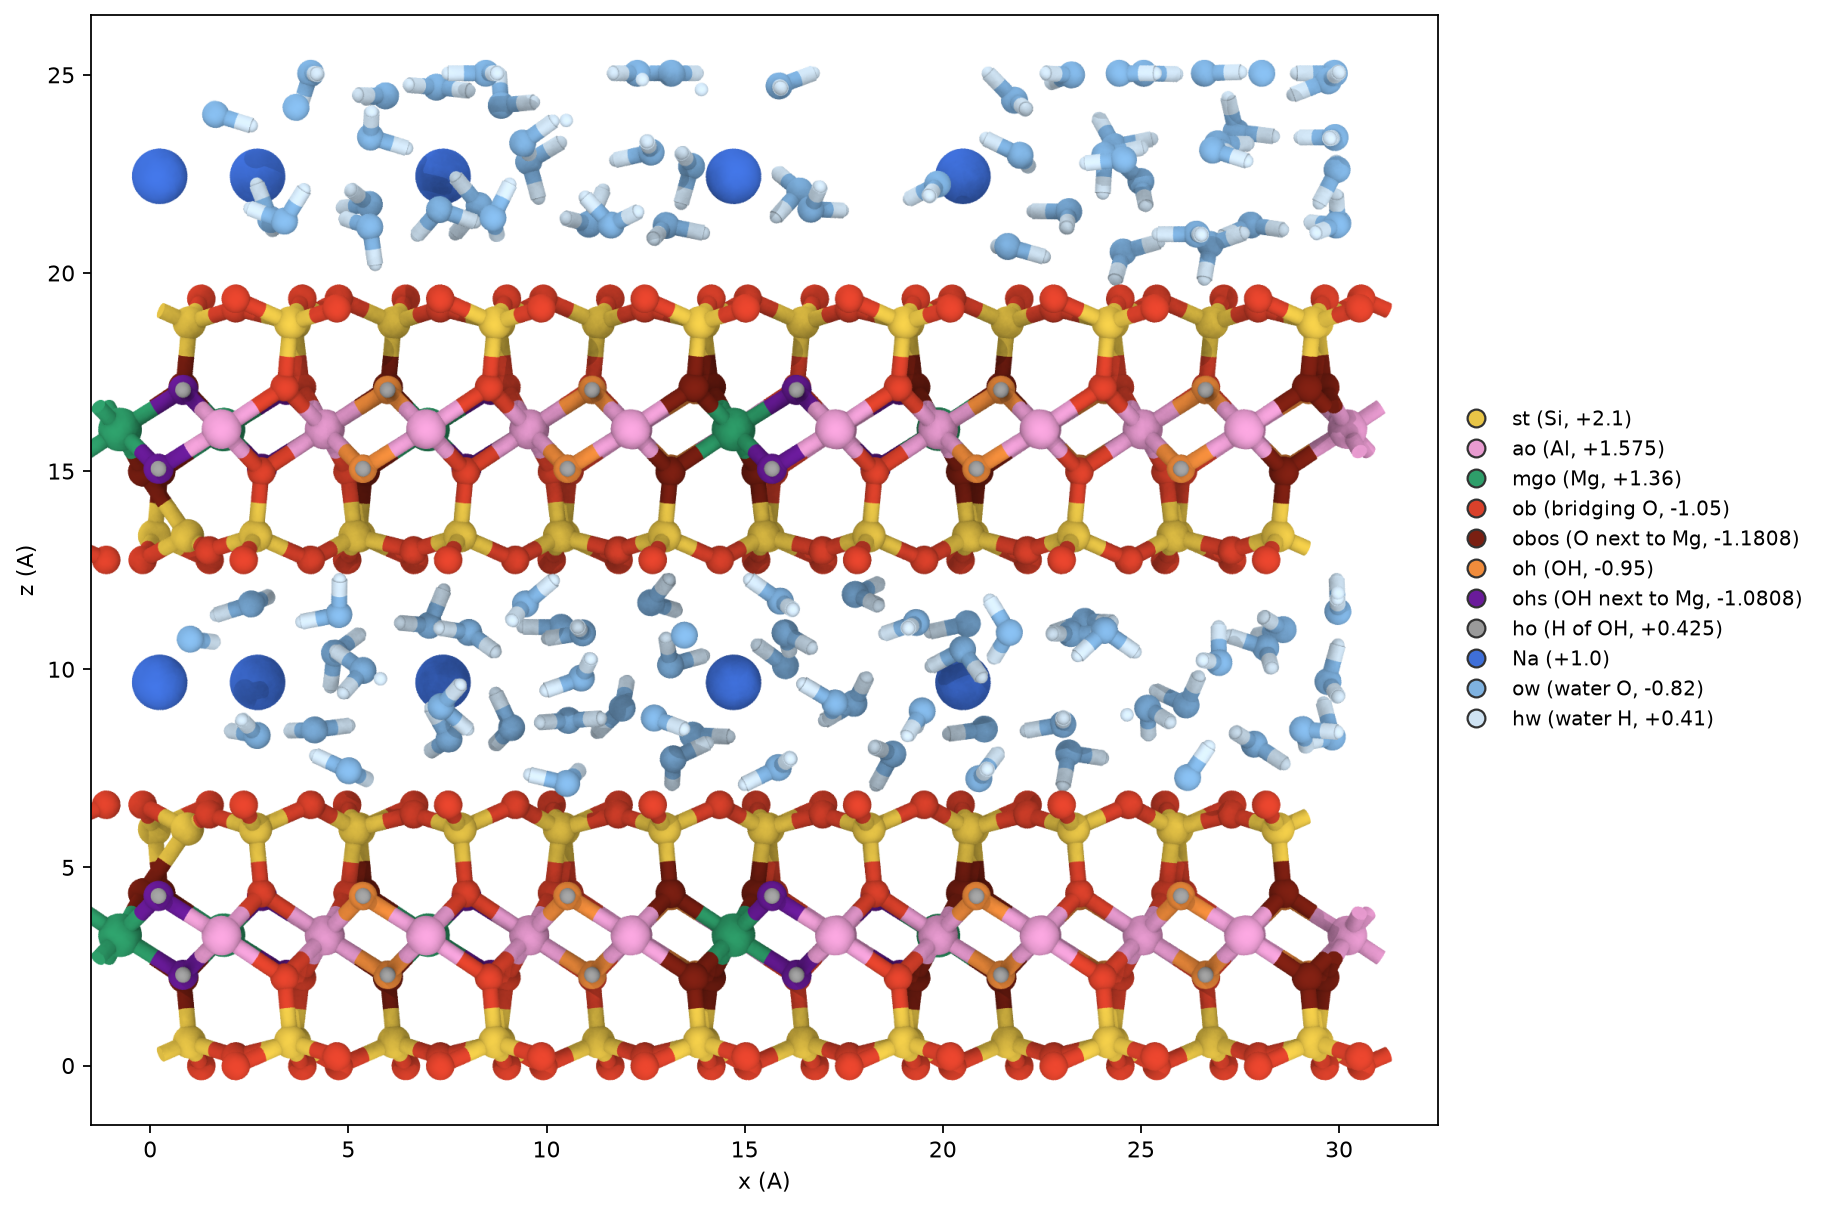
\includegraphics[width=0.85\linewidth]{figs/system.png}
\caption{Na モンモリロナイトの初期構造（OVITO\cite{ovito}による描画，セルの中央の厚さ 8\,\AA{} の切片）．色は ClayFF の型で，括弧内は電荷．}
\label{fig:system}
\end{figure}

\subsection{SOAP 記述子}
SOAP\cite{bartok2013}は，中心原子 $i$ のまわりの原子の配置を，回転と同種原子の入れ替えに対して不変なベクトルで表す．
カットオフ $r_\mathrm{c}$ 以内の元素 $Z$ の原子の位置に幅 $\sigma$ のガウス関数を置いて元素ごとの密度 $\rho_i^Z(\mathbf{r})$ を作り，動径の基底 $g_n(r)$（$n=1,\dots,n_{\max}$）と球面調和関数 $Y_{lm}$（$l=0,\dots,l_{\max}$）で展開する．
\begin{equation}
\rho_i^{Z}(\mathbf{r}) = \sum_{n,l,m} c^{Z}_{nlm}(i)\, g_n(r)\, Y_{lm}(\hat{\mathbf{r}})
\end{equation}
係数を $m$ について和をとり，回転不変なパワースペクトルにする．
\begin{equation}
p^{Z_1 Z_2}_{n n' l}(i) = \pi\sqrt{\frac{8}{2l+1}} \sum_{m=-l}^{l} c^{Z_1}_{nlm}(i)^{*}\, c^{Z_2}_{n'lm}(i)
\end{equation}
すべての元素の組，$n$，$n'$，$l$ の成分を並べたものが原子 $i$ の SOAP ベクトルである．
本稿では $r_\mathrm{c}=5$\,\AA，$n_{\max}=4$，$\sigma=0.4$\,\AA{} とし，元素は H, O, Na, Mg, Al, Si, K, Cs の 8 種である（Na モンモリロナイトだけの確認（表\ref{tab:loo}の上 2 行）では H, O, Na, Mg, Al, Si の 6 種）．
粘土の原子，水，Na$^+$ のすべてを中心原子とし，すべてを近くの原子として含める．
計算は dscribe\cite{dscribe} で行い，ベクトルは長さ 1 に正規化した．
2 つの配置の似かたは，ベクトルの内積（コサイン類似度）で測る．

\subsection{一対一の対応の確認}
初期構造の各原子について，同じ元素の別の原子のうち SOAP がいちばん似たもの（最近傍）を探し，その電荷が自分と同じかを調べた．
すべての原子で同じなら，SOAP から電荷を一意に決められる．
$l_{\max}$ は 3，4，5 とした（元素 6 種で次元は 1{,}200，1{,}500，1{,}800）．

\subsection{力場：ClayFF と SPC 水}
\label{sec:ff}
力場は，ClayFF の原論文 Cygan ら\cite{cygan2004}の表 1（非結合のパラメータ）と表 2（結合のパラメータ）のとおりである．
水は，ClayFF の柔軟な SPC 水（O--H の伸縮と H--O--H の変角を持つ）で，Na$^+$，K$^+$，Cs$^+$ のパラメータも ClayFF の表の値である．
SOAP が決めるのは各原子の電荷と型だけで，下に示す関数形とパラメータは型ごとに固定されている（LAMMPS の単位系 \texttt{real}，エネルギーは kcal/mol，距離は \AA）．

\paragraph{関数形．}
全ポテンシャルエネルギーは，非結合項と結合項の和である．
\begin{equation}
E = \sum_{i<j}\left\{ D_{0,ij}\left[\left(\frac{R_{0,ij}}{r_{ij}}\right)^{12}-2\left(\frac{R_{0,ij}}{r_{ij}}\right)^{6}\right] + \frac{C\,q_i q_j}{r_{ij}} \right\}
+ \sum_{\mathrm{O\text{--}H}} k_1 (r-r_0)^2 + \sum_{\mathrm{angles}} k_2(\theta-\theta_0)^2
\end{equation}
第 1 項は Lennard-Jones（12-6）で，$D_0$ と $R_0$ は表\ref{tab:ffparam}の値，異種の原子の間は $D_{0,ij}=\sqrt{D_{0,i}D_{0,j}}$，$R_{0,ij}=(R_{0,i}+R_{0,j})/2$ とする．
LAMMPS には $\varepsilon = D_0$，$\sigma = R_0/2^{1/6}$ として渡す（同じ関数である）．
第 2 項はクーロン力（$C = 332.0637$\,kcal\,\AA/(mol\,$e^2$)）である．
LJ と実空間のクーロン力のカットオフは 10\,\AA，LJ の遠距離の補正はなし，クーロン力の長距離部分は PPPM（相対精度 $10^{-5}$）で計算する．
結合している原子の間（O--H）と，同じ分子内で結合を 2 つ隔てた原子（H--O--H の H--H，M--O--H の M--H）の非結合の相互作用は除く．
結合項は，水と粘土の OH の O--H の伸縮（調和型，表\ref{tab:ffbond}）と，水の H--O--H の変角，OH の O に結合した陽イオン M と H の変角 M--O--H である（調和型，表\ref{tab:ffbond}）．
M--O--H は，Si を含めた骨格の陽イオンすべてに同じ係数（$k_2=30.0$\,kcal/(mol\,rad$^2$)，$\theta_0=109.47^\circ$）を使う．
SOAP の電荷を使うのは第 2 項の $q_i$ だけである．

\begin{table}[!htbp]
\centering
\caption{ClayFF の非結合のパラメータ（Cygan ら\cite{cygan2004}の表 1）．本稿の型の名前は，水の O（o*）を ow，水の H（h*）を hw とした．$D_0$ と $R_0$ は LJ の 12-6 の深さと極小の距離．Na$^+$ と Cs$^+$ は Smith と Dang\cite{smithdang}，K$^+$ は Koneshan ら\cite{koneshan1998}の値（Cygan ら\cite{cygan2004}の表 1 の注のとおり）．}
\label{tab:ffparam}
\small
\begin{tabular}{llrrr}
\toprule
型 & 種類 & 電荷（$e$） & $D_0$（kcal/mol） & $R_0$（\AA） \\
\midrule
hw（h*） & 水の H & $+0.4100$ & 0 & 0 \\
ho & OH の H & $+0.4250$ & 0 & 0 \\
ow（o*） & 水の O & $-0.8200$ & 0.1554 & 3.5532 \\
oh & OH の O & $-0.9500$ & 0.1554 & 3.5532 \\
ob & 架橋 O & $-1.0500$ & 0.1554 & 3.5532 \\
obos & 八面体の置換のある架橋 O & $-1.1808$ & 0.1554 & 3.5532 \\
obts & 四面体の置換のある架橋 O & $-1.1688$ & 0.1554 & 3.5532 \\
ohs & 置換のある OH の O & $-1.0808$ & 0.1554 & 3.5532 \\
st & 四面体の Si & $+2.1000$ & $1.8405\times10^{-6}$ & 3.7064 \\
at & 四面体の Al & $+1.5750$ & $1.8405\times10^{-6}$ & 3.7064 \\
ao & 八面体の Al & $+1.5750$ & $1.3298\times10^{-6}$ & 4.7943 \\
mgo & 八面体の Mg & $+1.3600$ & $9.0298\times10^{-7}$ & 5.9090 \\
mgh & 水酸化物の Mg & $+1.0500$ & $9.0298\times10^{-7}$ & 5.9090 \\
Na & 水溶液中の Na$^+$ & $+1.0$ & 0.1301 & 2.6378 \\
K & 水溶液中の K$^+$ & $+1.0$ & 0.1000 & 3.7423 \\
Cs & 水溶液中の Cs$^+$ & $+1.0$ & 0.1000 & 4.3002 \\
\bottomrule
\end{tabular}
\end{table}

\begin{table}[!htbp]
\centering
\caption{ClayFF の結合のパラメータ（Cygan ら\cite{cygan2004}の表 2）．伸縮は $k_1(r-r_0)^2$（kcal/(mol\,\AA$^2$)，\AA），変角は $k_2(\theta-\theta_0)^2$（kcal/(mol\,rad$^2$)，度）．M は骨格の陽イオン（Si，Al，Mg）．}
\label{tab:ffbond}
\small
\begin{tabular}{llcc}
\toprule
 & 原子 & $k$ & $r_0$ または $\theta_0$ \\
\midrule
伸縮 & ow--hw，oh--ho，ohs--ho & 554.1349 & 1.0000 \\
変角 & hw--ow--hw & 45.7696 & 109.47 \\
変角 & M--oh--ho，M--ohs--ho & 30.0 & 109.47 \\
\bottomrule
\end{tabular}
\end{table}

\paragraph{水のモデル．}
水は ClayFF の柔軟な SPC 水で，O の電荷 $-0.82\e$，H の電荷 $+0.41\e$，O の LJ は $D_0=0.1554$\,kcal/mol，$R_0=3.5532$\,\AA（H には LJ なし）である．
O--H の伸縮と H--O--H の変角は調和型で，剛体にはしない（SHAKE は使わない）．
そのため時間刻みは 0.5\,fs とした．
粘土の OH の O--H も，ClayFF のとおり柔軟な調和型である．

\paragraph{MD の条件．}
温度は Nosé--Hoover\cite{nose1984,hoover1985}の恒温槽（緩和時間 100\,fs），NPT では Nosé--Hoover の恒圧槽（緩和時間 1000\,fs）である．
最小化は共役勾配法で，1 回の移動量の上限を 0.01\,\AA，次に 0.1\,\AA{} として行う．

\subsection{力場の自動生成}
図\ref{fig:workflow}に流れを示す．
\paragraph{ライブラリ．}
参照の構造（\ref{sec:refs} 節）の全原子について，SOAP ベクトル（$l_{\max}=3$）と電荷と ClayFF の型を組にして保存する．
電荷は ClayFF の標準の値（表\ref{tab:ffparam}）で，SOAP に重みは付けず，参照を間引くこともしない．
元素 $e$ ごとに，SOAP ベクトルを行に並べた行列 $\mathbf{X}_e$ と，各行の電荷 $\mathbf{q}_e$ と型の組になる．
\paragraph{割り当て．}
入力は，元素と座標と箱だけの構造ファイル（extxyz，cif，POSCAR，LAMMPS のデータファイル）である．
その全原子の SOAP ベクトルの行列 $\mathbf{F}_e$ と類似度の行列 $\mathbf{S}_e = \mathbf{F}_e\mathbf{X}_e^{\mathsf{T}}$ の各行でいちばん大きい成分の列 $j^*$ を探し，その電荷 $q_{j^*}$ と型をそのまま与える（回帰も平均もしない）．
いちばん高い類似度が 0.95 未満の原子とライブラリにない元素の原子には，距離から決めた ClayFF の型とその電荷（水は SPC，イオンは形式電荷）を与えて記録する．
最後に，水の O に水の H がちょうど 2 個付く，水が中性，OH の O が H をちょうど 1 個持つ，などの分子と電荷の整合性を確かめ，合わないときは入力を書き出さずに原子を報告する．
あわせて，SOAP で決めた型を結合のつながりから決めた ClayFF の型と照らし合わせ（H のつき方が同じ型どうし，すなわち架橋 O どうし，OH の O どうし，陽イオンどうし），違う原子を報告する．
H のつき方が違う組を除くのは，水が鉱物に重なった初期構造では，結合のつながりの方が H の付いた O を読み違えるためである（Na モンモリロナイトの初期構造では 88 原子）．
この照合は，例えば白雲母を雲母のないライブラリで型付けすると，類似度が 0.95 以上でも四面体の Al に結合した O（obts）を ob と取り違えること（64 原子）を検出した（\ref{sec:ressheet} 節の金雲母の 16 原子も同じ）．
\paragraph{結合，角度，入力ファイル．}
結合と角度は，距離ではなく割り当てた型から決める（水の O は近い水の H を 2 つ，OH の H は近い OH の O を 1 つ取り，OH の O に結合した陽イオンと H の間に M--O--H を付ける）．
LJ，結合，角度の係数は ClayFF の表の値である（\ref{sec:ff} 節）．
入力ファイルは，エネルギー最小化，緩和の NVT（既定 10\,ps，記録しない），本計算の NVT，指定すれば NPT の順に MD を行う．
本計算では，水の O と各イオンの平均二乗変位（MSD）を LAMMPS の \texttt{compute msd} で 0.1\,ps ごとに書き出す．
全体の電荷が 0 でないときは，そのずれを粘土の原子に一様に配って中性にする．
\paragraph{解析．}
MD のあとの解析は，\texttt{compute msd} の MSD の直線部分の傾きからの拡散係数（Einstein の関係 $D=\lim\langle|\Delta\mathbf{r}|^2\rangle/(2dt)$，面内は $d=2$）と，SOVA\cite{sova}（sovapy）の二体分布関数（PDF）と動径分布関数（RDF）だけに限った．

\begin{figure}[!htbp]
\centering
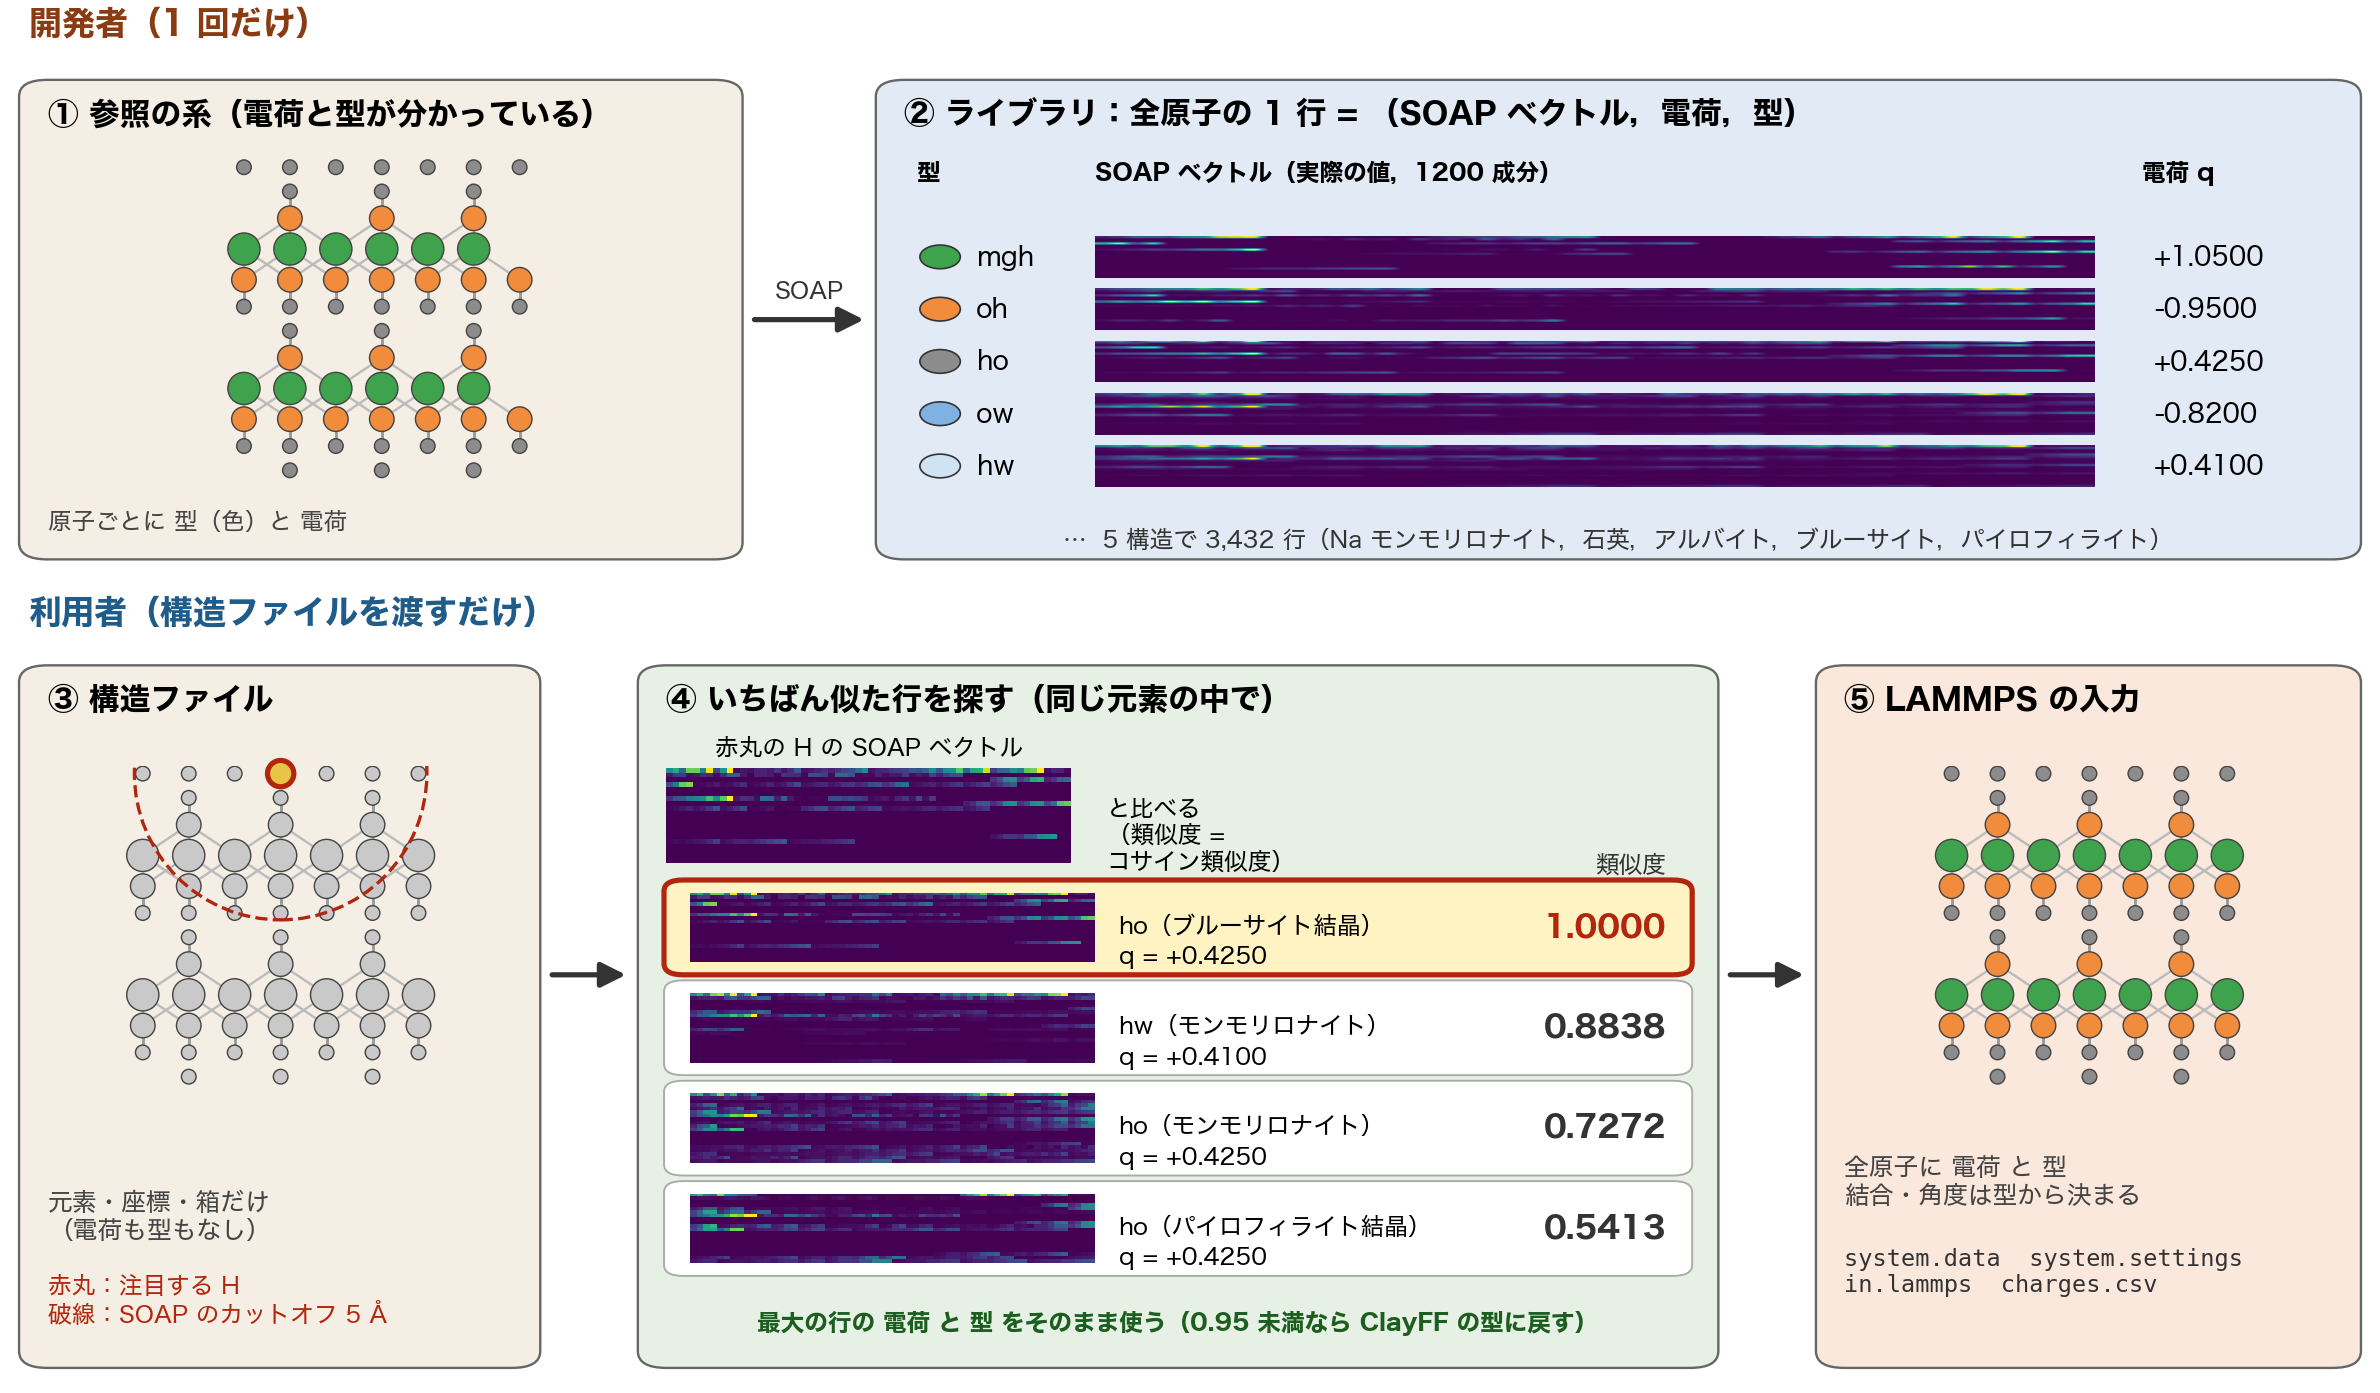
\includegraphics[width=\linewidth]{figs/workflow.png}
\caption{構造ファイルから LAMMPS 入力を作る流れ（実際のデータによる例）．上段は開発者が 1 回だけ行う作業で，① 電荷と型が分かっている参照の系（ここではブルーサイトの結晶，色は型）の全原子の SOAP ベクトルを計算し，② 1 原子を 1 行（型，SOAP ベクトル，電荷）とするライブラリにする．帯は SOAP ベクトルの実際の成分（1{,}200 成分を 20 $\times$ 60 に並べ，明るいほど大きい）．下段は利用者の作業で，③ 元素と座標と箱だけの構造ファイル（ここでは大きさの違うブルーサイトの結晶，灰色は型が未定）を渡すと，④ 各原子の SOAP ベクトルを同じ元素のライブラリの行と比べ（赤丸の H ではブルーサイトの ho との類似度 1.000 が最大で，水の H とは 0.88），いちばん似た行の電荷と型をそのまま付け，⑤ 結合と角度を型から決めて LAMMPS の入力を書き出す．}
\label{fig:workflow}
\end{figure}

\subsection{ソフトウェア：soapff-gui}
上の仕組みを，ウィンドウで操作する GUI ソフトウェア soapff-gui として実装した（Python の tkinter．SOAP は dscribe\cite{dscribe}，構造の読み書きは ASE\cite{ase}）．
利用者は，構造ファイルを選び，温度や MD の各段階の長さ，圧力などを必要なら変えて「実行」を押すだけでよい．
soapff-gui は，力場の作成（上の手順）で LAMMPS の入力一式（\texttt{system.data}，\texttt{system.settings}，\texttt{in.lammps}，原子ごとの型と電荷と類似度の表 \texttt{charges.csv}，\texttt{report.json}）を書き出し，LAMMPS を \texttt{mpirun} で起動して，段階（力場の作成，最小化，緩和の NVT，本計算），進み具合，温度，圧力，ポテンシャルエネルギー，密度と，SOAP で電荷を決めた原子と ClayFF の型に戻した原子の数，最小の類似度を表示する．
終わると，拡散係数と PDF・RDF の図と表を表示し，結果を OVITO\cite{ovito}で型ごとに色分けして開くこともできる．
LAMMPS を回さずに入力だけを書き出すこともできる．
力学物性は，入力（エネルギー最小化まで）のあとに「＋ 物性」で弾性定数（0\,K と有限温度），一軸の引張・圧縮，せん断を選ぶと，それぞれの LAMMPS のコマンドが入力の最後に追加され，計算のあとの解析で応力--ひずみ曲線と弾性定数の表が出る（\ref{sec:mechmethod} 節）．
これらは周期境界の構造なら鉱物の種類によらず同じ手順である．
ライブラリは，開発者が参照の構造から作って同梱する．
境界条件は x，y，z ごとに選べる（長距離のクーロン力は PPPM または MSM）が，本稿の計算はすべて 3 方向周期である．

\subsection{ライブラリの参照：Na モンモリロナイトと鉱物の結晶}
\label{sec:refs}
ライブラリの参照は，Na モンモリロナイトの初期構造（2{,}502 原子，水と Na$^+$ を含む）と，ClayFF の型で表せる 4 つの鉱物のバルクの結晶である（図\ref{fig:minerals}）．
結晶は，石英（SiO$_2$），骨格に Al(IV) と Na$^+$ を持つアルバイト（NaAlSi$_3$O$_8$），Mg の水酸化物であるブルーサイト（Mg(OH)$_2$），置換のない 2:1 型の粘土であるパイロフィライト（Al$_2$Si$_4$O$_{10}$(OH)$_2$）で，水を含まない．
石英，アルバイト，パイロフィライトは COD\cite{cod}の CIF（1011097，9000584，9000809）を ASE\cite{ase}で読んだ．
パイロフィライトの CIF には OH の H がないので，Al 2 個だけに結合した O（OH の O）から，2 個の Al と反対の向きに 0.97\,\AA{} の位置に H を置いた．
ブルーサイトは文献の結晶構造（$P\bar{3}m1$，$a=3.142$\,\AA，$c=4.766$\,\AA，H を含む）\cite{catti1995}から，ASE の空間群から結晶を作る関数で作った．
各辺が 10\,\AA{} 以上（SOAP のカットオフの 2 倍）になるように単位格子を繰り返した（石英 $3\times3\times2$，162 原子．アルバイト $2\times1\times2$，208 原子．ブルーサイト $4\times4\times3$，240 原子．パイロフィライト $2\times2\times2$，320 原子）．

ClayFF の型は，原子のまわりの結合のつながりから決める（Si--O 2.0\,\AA，Al--O 2.2\,\AA，Mg--O 2.4\,\AA，O--H 1.2\,\AA{} 以内を結合とする）．
石英は st と ob，アルバイトは st，at，ob，obts（Al(IV) に結合した架橋 O，$-1.1688\e$）と Na，ブルーサイトは mgh，oh，ho，パイロフィライトは st，ao，ob，oh，ho である．
電荷は，型ごとの ClayFF の標準の値（表\ref{tab:ffparam}）とした．
これらを LAMMPS のデータファイルとして書き出し，Na モンモリロナイトの初期構造（電荷を ClayFF の標準の値に付け替えたもの）と合わせて，まず 5 構造（3{,}432 原子，元素 H，O，Na，Mg，Al，Si）のライブラリを作った．
電荷の合計は，Na モンモリロナイトで $+0.006\e$，アルバイトで $-0.0032\e$，ほかは 0 である（ClayFF の標準の値の丸めによる）．
次に，層状ケイ酸塩の 8 つの結晶を加えた（表\ref{tab:sheet}）．
白雲母 2M$_1$ と 1M（KAl$_2$(AlSi$_3$)O$_{10}$(OH)$_2$），金雲母 1M（KMg$_3$(AlSi$_3$)O$_{10}$(OH)$_2$），Cs 雲母の nanpingite（CsAl$_2$(AlSi$_3$)O$_{10}$(OH)$_2$），1:1 型のカオリナイト（Al$_2$Si$_2$O$_5$(OH)$_4$）とリザーダイト（Mg$_3$Si$_2$O$_5$(OH)$_4$），タルク（Mg$_3$Si$_4$O$_{10}$(OH)$_2$），別の出典のパイロフィライトで，構造は共著者から提供された VASP の POSCAR である（タルクは Perdikatsis と Burzlaff の CIF\cite{perdikatsis1981}から作られたもの）．
白雲母 1M，nanpingite，リザーダイトの POSCAR には元素の行がないので，原子数の並びから元素の順を決め，配位数（Si は O が 4 個，八面体の Al と Mg は 6 個，四面体の Al は 4 個，H は 1.2\,\AA{} 以内に O が 1 個）で確かめた．
雲母の四面体の Al は at，それに結合した架橋 O は obts，層間の K$^+$ と Cs$^+$ は ClayFF の水溶液中のイオンの型（表\ref{tab:ffparam}）である．
金雲母，リザーダイト，タルクの三八面体の Mg は，八面体シートに Al がないので mgh（$+1.05\e$）とした（この型で電荷が中性になる）．
各辺が 10\,\AA{} 以上になるように単位格子を繰り返した（168--408 原子）．
電荷の合計は雲母で $-0.0016$ から $-0.0032\e$（obts の電荷の丸めによる），ほかは 0 である．
Fe$^{2+}$ の雲母の annite（KFe$_3$(AlSi$_3$)O$_{10}$(OH)$_2$）は，ClayFF の表に八面体の Fe$^{3+}$（feo）しかなく，標準の電荷で中性にならないので加えなかった．
こうして，ライブラリは 13 構造，5{,}878 原子（元素 H，O，Na，Mg，Al，Si，K，Cs）になった．
開発者の確認として，ライブラリの全原子について，ライブラリの中で SOAP がいちばん似た別の原子の電荷が同じかを調べた（ほかの構造の原子も含めて探す）．

\begin{figure}[!htbp]
\centering
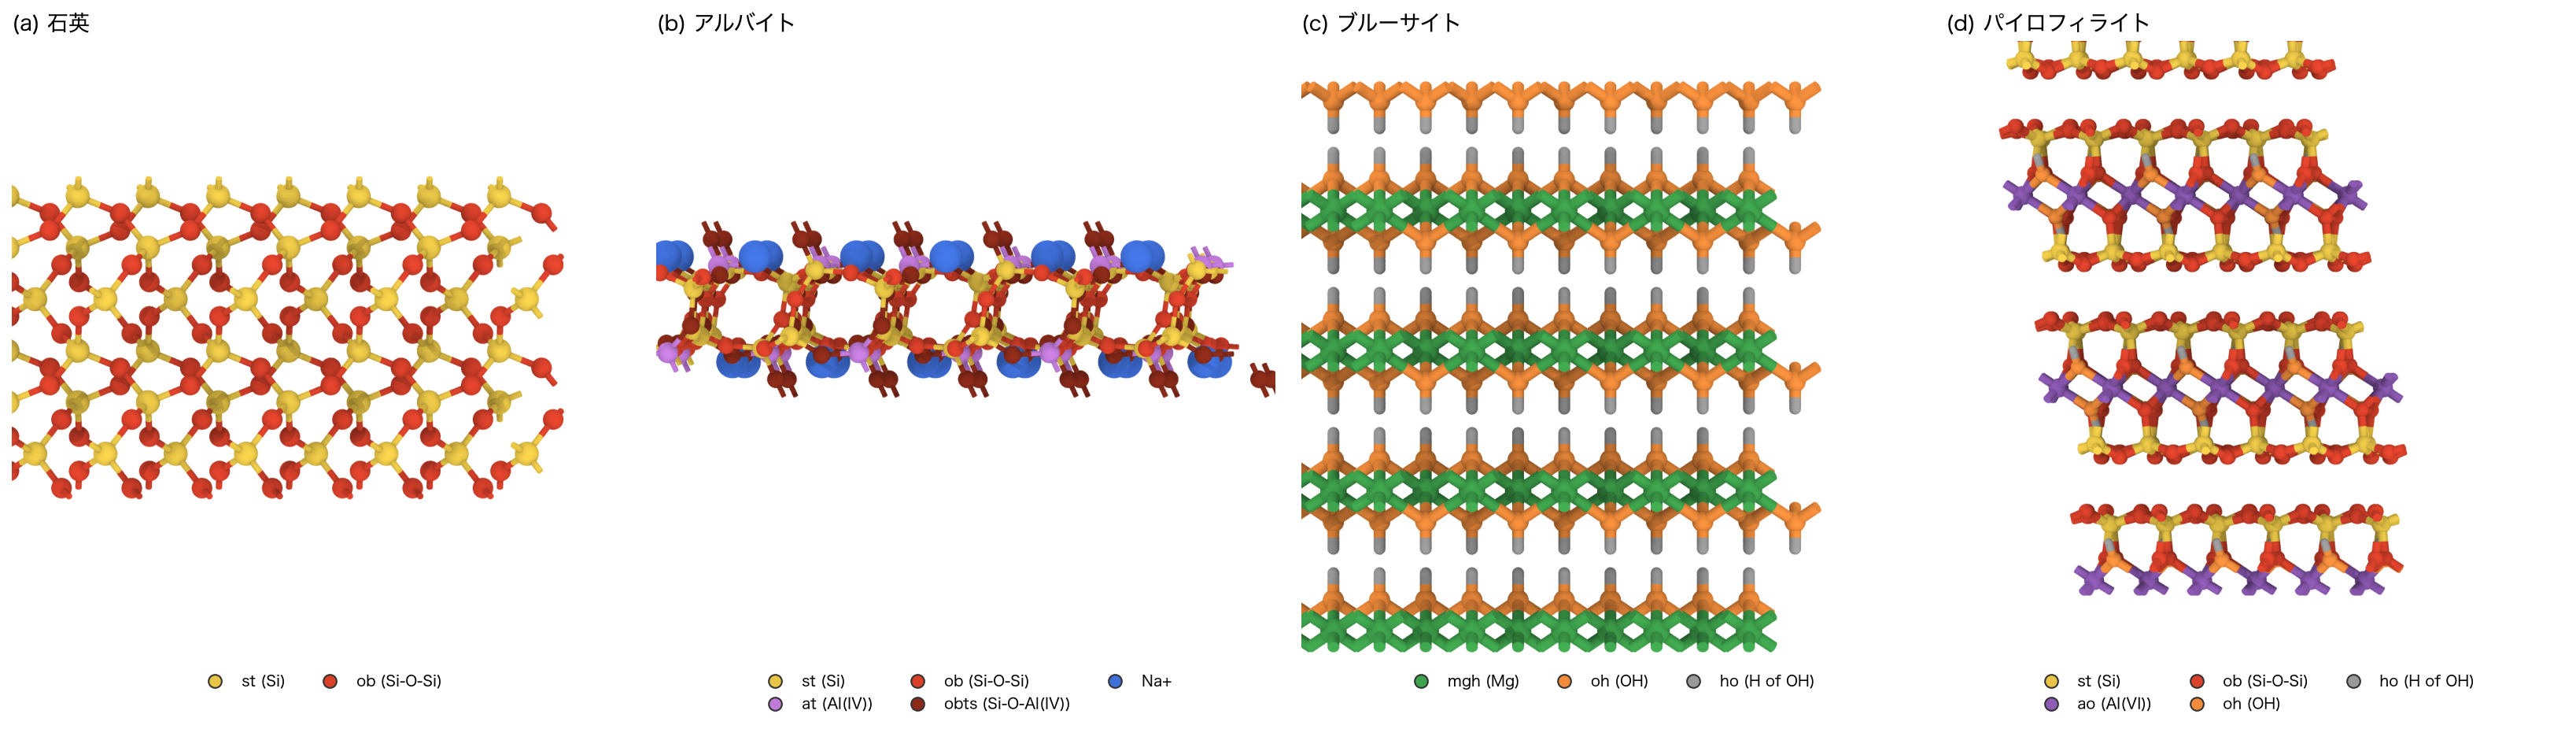
\includegraphics[width=\linewidth]{figs/minerals.png}
\caption{ライブラリの鉱物の結晶（OVITO\cite{ovito}による描画，構造ファイルから作った力場の型で色分け）．(a) 石英．(b) アルバイト．(c) ブルーサイト．(d) パイロフィライト．ライブラリより大きい超格子（試験の構造）．}
\label{fig:minerals}
\end{figure}

\subsection{Na モンモリロナイトの力場の試験}
初期構造（2{,}502 原子）を元素と座標と箱だけの extxyz に書き出し，ツールに渡した．
生成した電荷，型，結合，LJ パラメータを，ライブラリの作成に使ったラベル（ClayFF の標準の電荷と型）と比べ，生成した入力で LAMMPS\cite{lammps}を回した．
この構造はライブラリの参照そのものなので，これは構造ファイルから入力を作る手順（SOAP の計算，最近傍，結合と角度，入力の書き出し）が正しく働くかの確認である．

\subsection{ライブラリより大きい結晶での試験}
ライブラリにない構造でうまく働くかを調べるため，4 つの鉱物の結晶を，ライブラリとは違う大きさの超格子（石英 $4\times3\times2$，216 原子．アルバイト $3\times2\times1$，312 原子．ブルーサイト $5\times5\times4$，500 原子．パイロフィライト $3\times2\times3$，720 原子）で作り，元素と座標と箱だけにしてツールに渡した．
正解は，結合のつながりから決めた ClayFF の型と，その標準の電荷である．
型が正解と違うか，電荷が 0.01\e{} より大きく違う原子（誤り）を数え，各原子のいちばん高い類似度と，しきい値 0.95 未満で距離から決めた型に戻された原子（fallback）の数を調べた．

\subsection{層状ケイ酸塩の結晶での試験}
\label{sec:sheetmethod}
加えた 8 つの結晶について，3 つの試験を行った．
(1) ライブラリと大きさの違う超格子（a 方向に単位格子を 1 つ多く繰り返したもの，336--672 原子）をツールに渡し，型と電荷を正解（結合のつながりから決めた ClayFF の型と標準の電荷）と比べた．
(2) その力場で，最小化，300\,K の緩和の NVT 10\,ps，NVT 10\,ps，NPT（箱の全成分と傾き，1\,atm）40\,ps を回し，最後のフレーム（熱で乱れ，箱も変わった構造）をもう一度ツールに渡して，同じ正解と比べた．NPT の後半 30\,ps の平均の格子定数を，入力の構造と比べた．
(3) その鉱物の参照をライブラリから除いた 12 構造のライブラリで，(2) の最後のフレームを型付けし，ほかの鉱物の参照だけで正しく型付けできるかを調べた．
加えて，前の 5 構造のライブラリで行った試験（Na モンモリロナイトの初期構造，石英など 4 つの結晶の超格子）を，13 構造のライブラリでやり直した．

\subsection{MD の手順の確認}
結晶の超格子の 4 構造と Na モンモリロナイトの初期構造について，soapff-gui の既定の手順（最小化，300\,K で 10\,ps の緩和の NVT，本計算）で LAMMPS を回し，温度とポテンシャルエネルギーが安定するかを調べた．
結晶は，緩和の NVT のあと NVT 10\,ps，さらに NPT（箱の全成分と傾き，1\,atm）40\,ps を回し，実験の格子から箱の大きさがどれだけ変わるかも調べた．
Na モンモリロナイトの初期構造は，緩和の NVT，NVT 10\,ps，面に垂直な方向だけ箱が変わる NPT 100\,ps（圧力 1\,atm）を回した．

\subsection{拡散係数の先行研究との比較}
\label{sec:diffmethod}
生成した力場で得られる物性が先行研究と合うかを，Na モンモリロナイトの 2 水和層の層間の水と Na$^+$ の面内の拡散係数で調べた．
比較の対象は，同じ ClayFF と柔軟な SPC 水を用いて 2 水和層の拡散係数の温度依存性を求めた Greathouse ら\cite{greathouse2016}の値（層電荷 $0.75$\e{} / O$_{20}$(OH)$_4$ の高電荷モデル）である．
Greathouse らは，LAMMPS で 0.5\,fs の時間刻みを用い，300\,K（高電荷では 330，366\,K も）で，NVT 50\,ps のあと NPT（面に垂直な方向だけ箱が変わる，圧力 0）2500\,ps を回し，後半 2000\,ps の座標を 2\,fs ごとに保存して，毎フレームを時間の原点として平均した MSD を 150--250\,ps で直線で近似して $D$ を求めている．
本稿の系は，層電荷が $0.83$\e{}，水が O$_{20}$(OH)$_4$ あたり 9.6 分子で，Greathouse らの高電荷モデル（水 7.9 分子）より水が多い．
構造ファイルから作った力場（\ref{sec:resmont} 節）で，300\,K の緩和の NVT 10\,ps と NVT 10\,ps，面に垂直な方向だけ箱が変わる NPT 100\,ps（1\,atm）を回した構造から，300，330，366\,K のそれぞれで新しい速度を与え，NVT 20\,ps，NPT（面に垂直，圧力 0，Greathouse らと同じ）100\,ps で平衡化した．
そのあと，NPT を 200\,ps ずつ 4 区間続け，区間ごとに新しく \texttt{compute msd} を定義して時間の原点を区間の始めにした．
各区間の水の O と Na$^+$ の面内の MSD を 50--200\,ps で直線で近似して $D_{xy}$ を求め（$\langle\Delta x^2+\Delta y^2\rangle=4Dt$），4 区間の平均と標準誤差を求めた（合計 800\,ps，時間の原点は区間ごとに 1 つ）．
活性化エネルギー $E_\mathrm{a}$ は，$\ln D_{xy}$ を $1/T$ に対して直線で近似して求めた（Greathouse らの 3 つの温度の値にも同じ近似を行った）．

\subsection{白雲母の弾性定数と力学試験}
\label{sec:mechmethod}
生成した力場で得られる力学物性を，白雲母 2M$_1$ で調べた．
単位格子を $2\times2\times1$ に繰り返した結晶（672 原子，20.71 $\times$ 17.97 $\times$ 20.07\,\AA，$\beta=95.76^\circ$）の構造ファイルから soapff-gui で力場を作り（全原子 SOAP，類似度の最小値 1.000），「＋ 物性」で生成したコマンドで計算した．
座標軸は，x を a 軸，y を b 軸（単斜晶のユニーク軸），z を層に垂直にとった．
\paragraph{0\,K の弾性定数．}
LAMMPS の例（examples/ELASTIC）の方法による．
\texttt{fix box/relax}（箱の全成分と傾き，応力 0）と箱を固定した最小化を 4 回交互に行って応力が 0 の箱にした（残りの応力は各成分 $10^{-3}$\,GPa 未満）．
そこから 6 つのひずみ（xx，yy，zz，yz，xz，xy）をそれぞれ $\pm 0.005$ だけ箱に与え（\texttt{change\_box}，原子は箱とともに移す），箱を固定して原子を最小化し，応力テンソルの変化から $C_{ij} = -\left[p_i(+\varepsilon_j)-p_i(-\varepsilon_j)\right]/(2\varepsilon_j)$ を求めた（$p_i$ は LAMMPS の圧力テンソルの成分，応力 $=-$圧力）．
$C_{ij}$ を対称化し，Voigt，Reuss，Hill の体積弾性率とせん断弾性率，コンプライアンス $S=C^{-1}$ からヤング率 $E_x=1/S_{11}$ などを求めた．
ひずみの大きさは，最小化の収束で決めた．
PPPM の力では最小化が残りの応力 50--100\,atm ほどで止まり（線探索が進まなくなる），ひずみ $\pm10^{-3}$ では $C_{ij}$ が 5--10\,GPa ばらついた（計算機と並列数を変えると $C_{33}$ が 68 と 79\,GPa，$C_{44}$ が 16 と 19\,GPa）．
ひずみ $\pm0.005$ と $\pm0.01$ では，$C_{ij}$ は 2 GPa 以内で一致し，並列数（2，4）によらず，$C_{ij}$ と $C_{ji}$ の差も 2\,GPa 以下だったので，$\pm0.005$ を用いた（soapff-gui の既定値）．
\paragraph{300\,K の引張とせん断．}
soapff-gui で構造ファイルから力場を作り，「＋ 物性」で 0\,K の弾性定数，x，y，z の引張，xy，xz，yz のせん断を選んで生成した入力を，そのまま SSH で別の計算機（8 並列，LAMMPS 7 Feb 2024）で回した（全体で 19 分）．
300\,K で緩和の NVT 10\,ps，NPT（箱の全成分と傾き，1\,atm）20\,ps を回し，箱を NPT の後半 10\,ps の平均にして平衡化した状態を保存した．
引張は，その状態から x，y，z のそれぞれに \texttt{fix deform} で一定のひずみ速度 $10^{9}$\,s$^{-1}$ で最大ひずみ 0.16 まで伸ばし，残りの 2 方向は \texttt{fix npt} で 1\,atm に保った．
せん断は，同じ状態から傾き（xy，xz，yz）を \texttt{fix deform} でひずみ速度 $10^{9}$\,s$^{-1}$ で最大 0.20 まで変え，\texttt{fix nvt} で 300\,K に保った．
応力は圧力テンソルの符号を変えたもので，100 ステップ（50\,fs）ごとに平均して記録した．
ヤング率とせん断弾性率はひずみ 0.02 までの応力--ひずみの傾き，強度は応力の最大値（100 ステップごとの記録を 0.5\,ps で移動平均したもの），破断ひずみは応力が最大の 70\,\% 未満に下がったひずみ，ポアソン比 $\nu_{ij}=-\varepsilon_i/\varepsilon_j$（$j$ の向きに引っ張ったときの $i$ の向きのひずみ）はひずみ 0.02 までの傾きである．
\paragraph{計算コードの確認．}
「＋ 物性」が生成するコマンドと解析が正しいかを，結果の分かっている計算で確かめた．
(1) 有限温度の弾性定数（\texttt{compute born/matrix} と応力のゆらぎ）は，LAMMPS の例（examples/ELASTIC\_T/BORN\_MATRIX/Argon，fcc の Ar，60\,K）に本稿の出力を加えて回し，解析の値をスクリプトが出す値と比べた．
$C_{11}$，$C_{12}$ は 2.455，1.299\,GPa（例 2.457，1.300\,GPa）で一致した．
$C_{44}$ は 1.494\,GPa（例 1.443\,GPa）だったが，例のスクリプトは yz の応力のゆらぎに xy の応力の平均を使っており，同じ取り違えをすると 1.443\,GPa になった．
(2) グリーン--久保の粘度と熱伝導率の単位は，固体の Ar（70\,K）で，LAMMPS のマニュアルの例のスクリプトが \texttt{trap()} で求めた値と比べ，$1.2066\times10^{-4}$ と $1.2074\times10^{-4}$\,Pa\,s，0.2762 と 0.2768\,W/(m\,K)（差は，温度に目標値と平均値のどちらを使うかと，kcal の換算（4186 と 4184\,J）の違いによる）で一致した．
(3) 0\,K の弾性定数は，石英の結晶で，弾性定数から求めた体積弾性率（184\,GPa）が，箱を等方に伸縮して最小化した圧力と体積の関係（185\,GPa）とエネルギーと体積の関係（186\,GPa）から独立に求めた値と一致した．
(4) 0\,K の弾性定数のひずみの大きさは，上に述べたとおり $\pm0.005$ と $\pm0.01$ で一致することで決めた．
(5) 引張とせん断は，同じ構造ファイルから 2 台の計算機（4 並列と 8 並列）で別々に回した結果が 3\,\% 以内で一致した．

\paragraph{比較．}
実験はブリルアン散乱による天然の白雲母の 13 の弾性定数（Vaughan と Guggenheim\cite{vaughan1986}）である（同じ座標軸）．
ClayFF による先行研究は 2 つである．
Teich-McGoldrick ら\cite{teich2012}は，Kuwahara の構造から作った白雲母 2M$_1$（四面体の Al は Loewenstein 則に従って Si$_4$Al$_2$ と Si$_5$Al$_1$ の環が同数，$8\times4\times2$，5{,}376 原子，Ewald 法，時間刻み 1\,fs）で，0\,K の静的な方法（ひずみ $5\times10^{-7}$）による 13 の弾性定数と，298，500，800\,K でひずみ速度 $10^{8}$\,s$^{-1}$ の引張・圧縮とせん断の応力--ひずみ曲線から，ヤング率，せん断弾性率，ポアソン比を求めた．
DelRio ら\cite{delrio2026}は，白雲母のマイクロスケールのせん断試験による破壊靭性の温度依存性を調べ，あわせて MD で x，y，z の引張の応力--ひずみ曲線を 25--400\,$^\circ$C で求めた（x，y の破断応力は約 12\,GPa，z は約 3\,GPa で，温度とともに破断応力と破断ひずみが下がる）．
本稿と両者は，同じ ClayFF の型と電荷を使うが，Al の配置，系の大きさ，長距離のクーロン力の方法（本稿は PPPM），時間刻み（本稿は 0.5\,fs），ひずみ速度が違う．

\section{結果}
\subsection{水と Na$^+$ を含めた一対一の対応}
Na モンモリロナイトの初期構造の全原子（2{,}502 個）で，$l_{\max}=3$，4，5 のどれでも，最近傍の電荷が自分と同じだった（表\ref{tab:loo}）．
電荷が 0.13\e{} 違う ob と obos，oh と ohs だけでなく，水の O と粘土の O，水の H と OH の H も取り違えなかった．
石英，アルバイト，ブルーサイト，パイロフィライトの結晶を加えた 5 構造のライブラリ（3{,}432 原子）でも，全原子で最近傍の電荷が自分と同じで（$l_{\max}=3$，4，5），ブルーサイトの Mg（mgh，1.05\e）とモンモリロナイトの八面体の Mg（mgo，1.36\e），Si--O--Si の O（ob）と Si--O--Al の O（obts）も区別された．
層状ケイ酸塩の 8 つの結晶を加えた 13 構造のライブラリ（5{,}878 原子，元素 8 種）でも，$l_{\max}=3$，4，5 のどれでも全原子で最近傍の電荷が自分と同じだった．
したがって，水と Na$^+$ を含めても，鉱物の結晶を加えても，ライブラリのすべての原子で SOAP と電荷は一対一に対応する．

\begin{table}[!htbp]
\centering
\caption{ライブラリの中での一対一の確認（最近傍の電荷が自分と同じ原子の数）．Na モンモリロナイトは水と Na$^+$ を含む全原子，ライブラリ全体は鉱物の結晶を加えたもの．カットオフ 5\,\AA．}
\label{tab:loo}
\small
\begin{tabular}{lccc}
\toprule
対象 & $l_{\max}=3$ & $l_{\max}=4$ & $l_{\max}=5$ \\
\midrule
粘土の原子（Na モンモリロナイトのうち） & 1{,}440 / 1{,}440 & 1{,}440 / 1{,}440 & 1{,}440 / 1{,}440 \\
Na モンモリロナイト（本稿，水と Na$^+$ を含む） & 2{,}502 / 2{,}502 & 2{,}502 / 2{,}502 & 2{,}502 / 2{,}502 \\
ライブラリ全体（5 構造） & 3{,}432 / 3{,}432 & 3{,}432 / 3{,}432 & 3{,}432 / 3{,}432 \\
ライブラリ全体（層状ケイ酸塩を加えた 13 構造） & 5{,}878 / 5{,}878 & 5{,}878 / 5{,}878 & 5{,}878 / 5{,}878 \\
\bottomrule
\end{tabular}
\end{table}

\subsection{構造ファイルから作った力場}
\label{sec:resmont}
Na モンモリロナイトの初期構造の構造ファイルから作った力場では，2{,}502 原子のすべてで電荷と型がライブラリのラベルと一致した（表\ref{tab:types}）．
すべての原子が SOAP で決まり（類似度 1.0），fallback になった原子はなかった．
粘土 1{,}440 原子，水 1{,}032 原子（344 分子），Na$^+$ 30 原子に分かれ，電荷の合計は $+0.006\e$ から $10^{-13}\e$ 以下に補正された（補正は粘土の原子 1 個あたり $4\times10^{-6}\e$）．
結合は 832（OH 144，水の O--H 688），角度は水の H--O--H 344 と M--O--H 288（計 632）である．
LJ パラメータは表\ref{tab:ffparam}の値（$\varepsilon=D_0$，$\sigma=R_0/2^{1/6}$）と一致した．

\begin{table}[!htbp]
\centering
\caption{構造ファイルから作った Na モンモリロナイトの力場の型ごとの原子数，電荷，LJ パラメータ．電荷と LJ は表\ref{tab:ffparam}の ClayFF の値で，電荷はすべての原子でライブラリのラベルと一致した．}
\label{tab:types}
\small
\begin{tabular}{llrrrr}
\toprule
型 & 中身 & 原子数 & 電荷（$e$） & $D_0$（kcal/mol） & $R_0$（\AA） \\
\midrule
st & 四面体の Si & 288 & $+2.1000$ & $1.8405\times10^{-6}$ & 3.7064 \\
ao & 八面体の Al & 114 & $+1.5750$ & $1.3298\times10^{-6}$ & 4.7943 \\
mgo & 八面体の Mg（置換） & 30 & $+1.3600$ & $9.0298\times10^{-7}$ & 5.9090 \\
ob & 架橋 O & 600 & $-1.0500$ & 0.1554 & 3.5532 \\
obos & Mg に結合した架橋 O & 120 & $-1.1808$ & 0.1554 & 3.5532 \\
oh & Al$_2$--OH の O & 84 & $-0.9500$ & 0.1554 & 3.5532 \\
ohs & Mg に結合した OH の O & 60 & $-1.0808$ & 0.1554 & 3.5532 \\
ho & OH の H & 144 & $+0.4250$ & 0 & 0.0000 \\
Na & 層間の Na$^+$ & 30 & $+1.0000$ & 0.1301 & 2.6378 \\
ow & 水の O & 344 & $-0.8200$ & 0.1554 & 3.5532 \\
hw & 水の H & 688 & $+0.4100$ & 0 & 0.0000 \\
\bottomrule
\end{tabular}

\end{table}

\subsection{ライブラリより大きい結晶}
ライブラリより大きい超格子の 4 つの結晶（216--720 原子）では，すべての原子で型と電荷が正解（結合のつながりから決めた ClayFF の型と標準の電荷）と一致した（表\ref{tab:bulk}）．
すべての原子の類似度は 1.000 で，しきい値 0.95 未満の原子（fallback）はなく，分子と電荷の整合性の確認で止まった構造もなかった．
超格子の中の各原子のまわり 5\,\AA{} の環境が，ライブラリの結晶の中の同じ型の原子と同じだったためである．
石英の ob，アルバイトの ob と obts，Na，ブルーサイトの mgh，oh，ho，パイロフィライトの ao，oh，ho が，いずれも正しく付いた．

\begin{table}[!htbp]
\centering
\caption{ライブラリより大きい超格子の結晶での結果．「誤り」は型が正解と違うか電荷が 0.01\e{} より大きく違う原子の数，「最小類似度」は全原子のいちばん高い類似度の最小値，fallback は類似度 0.95 未満で距離から決めた型に戻された原子の数．}
\label{tab:bulk}
\small
\begin{tabular}{lrrrcc}
\toprule
鉱物 & 超格子 & 原子数 & 誤り & fallback & 最小類似度 \\
\midrule
石英 & $4\times3\times2$ & 216 & 0 & 0 & 1.000 \\
アルバイト & $3\times2\times1$ & 312 & 0 & 0 & 1.000 \\
ブルーサイト & $5\times5\times4$ & 500 & 0 & 0 & 1.000 \\
パイロフィライト & $3\times2\times3$ & 720 & 0 & 0 & 1.000 \\
\bottomrule
\end{tabular}
\end{table}

\subsection{層状ケイ酸塩の結晶}
\label{sec:ressheet}
層状ケイ酸塩の 8 つの結晶では，3 つの試験のどれでも，全原子の型と電荷が正解と一致した（表\ref{tab:sheet}）．
(1) ライブラリと大きさの違う超格子（336--672 原子）では，全原子の類似度が 1.000 だった．
(2) 300\,K の NVT と NPT のあとの最後のフレームでは，類似度の最小値は 0.962--0.988 に下がったが，すべてしきい値 0.95 以上で SOAP から決まり（fallback 0），誤りはなかった．
白雲母の obts（$-1.1688\e$）と ob（$-1.05\e$），oh と ohs，金雲母とタルクとリザーダイトの mgh，雲母の at と ao も区別された．
(3) その鉱物の参照を除いたライブラリでは，8 つのうち 7 つで誤りがなかった．
白雲母 2M$_1$，白雲母 1M，タルク，パイロフィライトは，ほかの鉱物の参照だけで，すべての原子が類似度 0.96 以上で型付けされた（ライブラリに同じ種類の層をもつ鉱物が残っているため）．
カオリナイトとリザーダイトは一部の原子（90，144 原子）が類似度 0.95 未満で fallback になったが，距離から決めた型も正しかった．
nanpingite の Cs$^+$ はほかの参照に Cs がないので類似度 0 で fallback になり，ClayFF の Cs の型が付いた．
一方，金雲母では，四面体の Al と 3 個の Mg（mgh）に結合した O の 16 原子が，obts でなく ob になった（電荷の差 0.12\e）．
この環境（Al(IV) と三八面体の Mg に囲まれた O）は，ほかの参照にない．
前の 5 構造のライブラリで行った試験も，13 構造のライブラリで結果は変わらなかった（Na モンモリロナイトの初期構造 2{,}502 原子，石英など 4 つの結晶の超格子 216--720 原子で誤り 0，類似度 1.000）．

\begin{table}[!htbp]
\centering
\caption{層状ケイ酸塩の結晶での試験．原子数はライブラリの参照と試験の超格子．(1) 大きさの違う超格子，(2) 300\,K の MD（NVT と NPT）のあとの最後のフレーム，(3) その鉱物の参照を除いたライブラリでの (2) のフレームの，誤り（型が違うか電荷が 0.01\e{} より違う原子）の数．括弧内は (2) の類似度の最小値と，(3) で fallback になった原子の数．}
\label{tab:sheet}
\small
\begin{tabular}{llrrccc}
\toprule
鉱物 & 型 & \multicolumn{2}{c}{原子数} & (1) & (2) & (3) \\
 & & 参照 & 試験 & & & \\
\midrule
白雲母 2M$_1$ & st at ao ob obts oh ho K & 336 & 672 & 0 & 0（0.962） & 0 \\
白雲母 1M & 同上 & 168 & 336 & 0 & 0（0.986） & 0 \\
金雲母 1M & st at mgh ob obts oh ho K & 176 & 352 & 0 & 0（0.976） & 16 \\
nanpingite & st at ao ob obts oh ho Cs & 336 & 504 & 0 & 0（0.967） & 0（24） \\
カオリナイト & st ao ob oh ho & 408 & 544 & 0 & 0（0.962） & 0（90） \\
リザーダイト & st mgh ob oh ho & 324 & 432 & 0 & 0（0.976） & 0（144） \\
タルク & st mgh ob oh ho & 378 & 504 & 0 & 0（0.980） & 0 \\
パイロフィライト（別の出典） & st ao ob oh ho & 320 & 480 & 0 & 0（0.988） & 0 \\
\bottomrule
\end{tabular}
\end{table}

\subsection{LAMMPS での MD}
Na モンモリロナイトの初期構造から作った入力は，そのまま LAMMPS で回った（図\ref{fig:md}）．
水が粘土に重なった初期構造でも，最小化のあと 300\,K の緩和の NVT 10\,ps で温度は 272--312\,K（後半の平均 299\,K），NVT 10\,ps で 293--312\,K（平均 299\,K）に収まった．
初期構造の箱は平衡化した構造より小さく，最小化のあとの圧力は約 $4.5\times10^4$\,atm と高いが，面に垂直な方向だけ箱が変わる NPT（1\,atm）で，層間距離 $d_{001}=L_z/2$ は 12.8\,\AA{} から 5\,ps ほどで 15.3\,\AA{} に広がり，その後 15.2--15.4\,\AA{} で一定だった．
ポテンシャルエネルギーは NPT の最初の 40\,ps ほどで下がり，以降 0.03\,kcal/mol/原子 以内で一定だった．
最後の 20\,ps の全体の圧力は約 $6\times10^3$\,atm で，x，y の箱の長さは固定しているため 1\,atm にはならない．

\begin{figure}[!htbp]
\centering
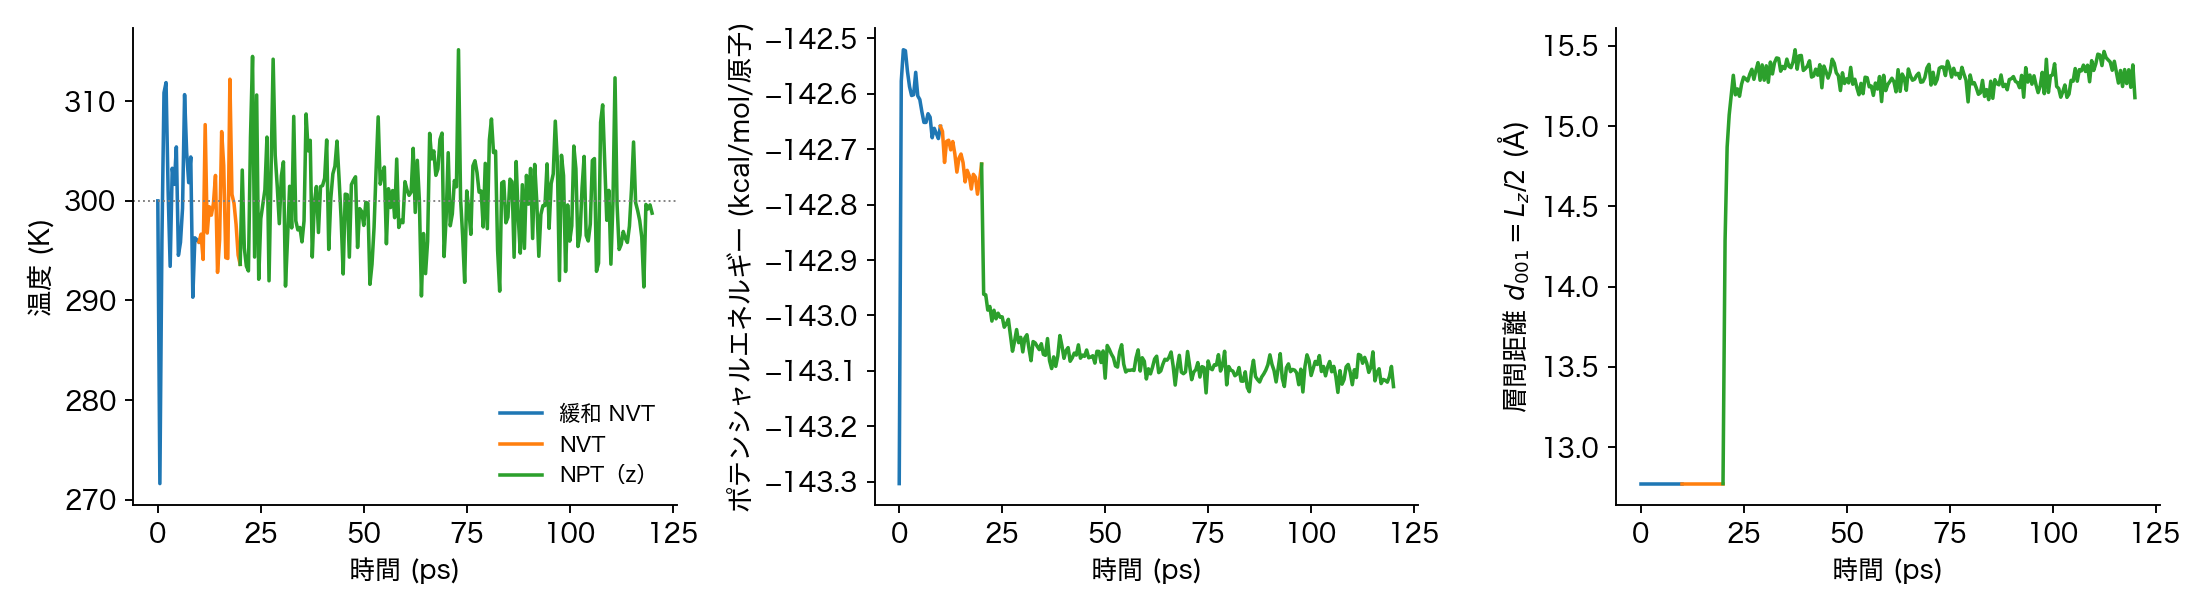
\includegraphics[width=\linewidth]{figs/md.png}
\caption{Na モンモリロナイトの初期構造から作った入力による MD（300\,K）：緩和の NVT 10\,ps，NVT 10\,ps，NPT（面に垂直な方向，1\,atm）100\,ps の，温度（左），原子あたりのポテンシャルエネルギー（中），層間距離 $d_{001}$（右）．}
\label{fig:md}
\end{figure}

ライブラリより大きい 4 つの結晶と層状ケイ酸塩の 8 つの結晶も，最小化，緩和の NVT，NVT を経て，NPT（箱の全成分と傾き，1\,atm）まで安定に回った（表\ref{tab:bulkmd}）．
温度は 270--338\,K で，NVT の平均は 300--302\,K だった．
実験の格子の箱のままの NVT の圧力は，石英 $+5.3$\,GPa，アルバイト $-5.3$\,GPa，ブルーサイト $+5.7$\,GPa，パイロフィライト $+1.9$\,GPa で，鉱物ごとに符号も大きさも違う．
NPT で箱を緩めると，後半 20\,ps の平均の体積は実験の格子から石英で $+4.9$\,\%，ブルーサイトで $+9.1$\,\%，パイロフィライトで $+2.0$\,\% 大きく，アルバイトで $-10.3$\,\% 小さくなった．
層状ケイ酸塩では，NPT の後半 30\,ps の平均の格子定数は，入力の構造から a，b で $-1.6$ から $+1.4$\,\%，c で $-4.8$ から $+2.7$\,\% 違い，体積の変化は $-7.1$ から $+3.7$\,\% だった．
白雲母 2M$_1$ は a，b，c が $+0.01$，$-0.26$，$-1.49$\,\%（体積 $-1.8$\,\%），層の間隔 $d_{001}=c\sin\beta/2$ は 9.99 から 9.83\,\AA{} になった．
白雲母 1M の $c$ の $-4.8$\,\% は，入力の構造の $d_{001}$（10.27\,\AA）が 2M$_1$ の入力（9.99\,\AA）より大きいためで，MD の $d_{001}$ は 1M で 9.80\,\AA，2M$_1$ で 9.83\,\AA{} とそろった．
角度は，カオリナイトの $\alpha$（$+4.6^\circ$）と $\beta$（$-2.2^\circ$），パイロフィライトの $\beta$（$-2.3^\circ$），タルクの $\alpha$（$+1.8^\circ$）を除いて $1^\circ$ 以内だった．
これらの差は ClayFF の性質で，SOAP の割り当てによるものではない（割り当てた型と電荷は正解と一致しており，力場は結合のつながりから手で型を決めたものと同じである）．

\begin{table}[!htbp]
\centering
\caption{ライブラリより大きい結晶の MD（300\,K，0.5\,fs）．NVT は入力の格子の箱で 10\,ps，NPT は箱の全成分と傾きを 1\,atm で 40\,ps．温度と圧力は NVT の平均，NPT の体積変化は後半（上 4 つは 20\,ps，層状ケイ酸塩は 30\,ps）の平均の，入力の格子の体積に対する割合．}
\label{tab:bulkmd}
\small
\begin{tabular}{lrccc}
\toprule
鉱物 & 原子数 & NVT の温度（K） & NVT の圧力（GPa） & NPT の体積変化（\%） \\
\midrule
石英 & 216 & 301 & $+5.3$ & $+4.9$ \\
アルバイト & 312 & 302 & $-5.3$ & $-10.3$ \\
ブルーサイト & 500 & 302 & $+5.7$ & $+9.1$ \\
パイロフィライト & 720 & 300 & $+1.9$ & $+2.0$ \\
\midrule
白雲母 2M$_1$ & 672 & 303 & $-0.68$ & $-1.8$ \\
白雲母 1M & 336 & 300 & $-4.37$ & $-7.1$ \\
金雲母 1M & 352 & 298 & $-0.88$ & $+0.8$ \\
nanpingite & 504 & 301 & $-3.02$ & $-4.3$ \\
カオリナイト & 544 & 302 & $+0.96$ & $+0.9$ \\
リザーダイト & 432 & 300 & $+3.06$ & $+3.7$ \\
タルク & 504 & 298 & $+1.33$ & $+2.9$ \\
パイロフィライト（別の出典） & 480 & 299 & $+1.91$ & $+2.1$ \\
\bottomrule
\end{tabular}
\end{table}

\subsection{拡散係数の先行研究との比較}
\label{sec:resdiff}
300，330，366\,K の平衡化のあとの層間距離 $d_{001}$ は 15.31，15.43，15.63\,\AA{} だった．
水の O の面内の拡散係数は，300\,K で $11.7\pm0.9$，330\,K で $18.3\pm0.5$，366\,K で $32.5\pm1.5$（$10^{-10}$\,m$^2$/s，4 区間の平均と標準誤差）で，Greathouse ら\cite{greathouse2016}の 13.1，24.3，39.4 の 0.90，0.75，0.82 倍だった（図\ref{fig:diffusion}）．
Na$^+$ は $4.3\pm0.9$，$10.3\pm0.7$，$15.3\pm4.7$ で，Greathouse らの 5.1，10.4，17.0 の 0.83，0.99，0.90 倍だった．
Na$^+$ は区間ごとのばらつきが大きい（366\,K で 7.2--28.1）．
活性化エネルギーは，水の O で $14.1\pm1.1$\,kJ/mol，Na$^+$ で $17.8\pm3.9$\,kJ/mol で，Greathouse らの 15.2，16.5\,kJ/mol（同じ近似では 15.2，16.7\,kJ/mol）と誤差の範囲で一致した．
拡散係数がやや小さいのは，本稿の系の層電荷（$0.83$\e）が Greathouse らの高電荷モデル（$0.75$\e）より大きく Na$^+$ が多いこと，平均の時間（800\,ps，区間ごとに時間の原点が 1 つ）が Greathouse らの 2000\,ps（2\,fs ごとの多数の時間の原点）より短いこと，有限サイズの補正をしていないことによると考えられる（両者とも補正なし）．

\begin{figure}[!htbp]
\centering
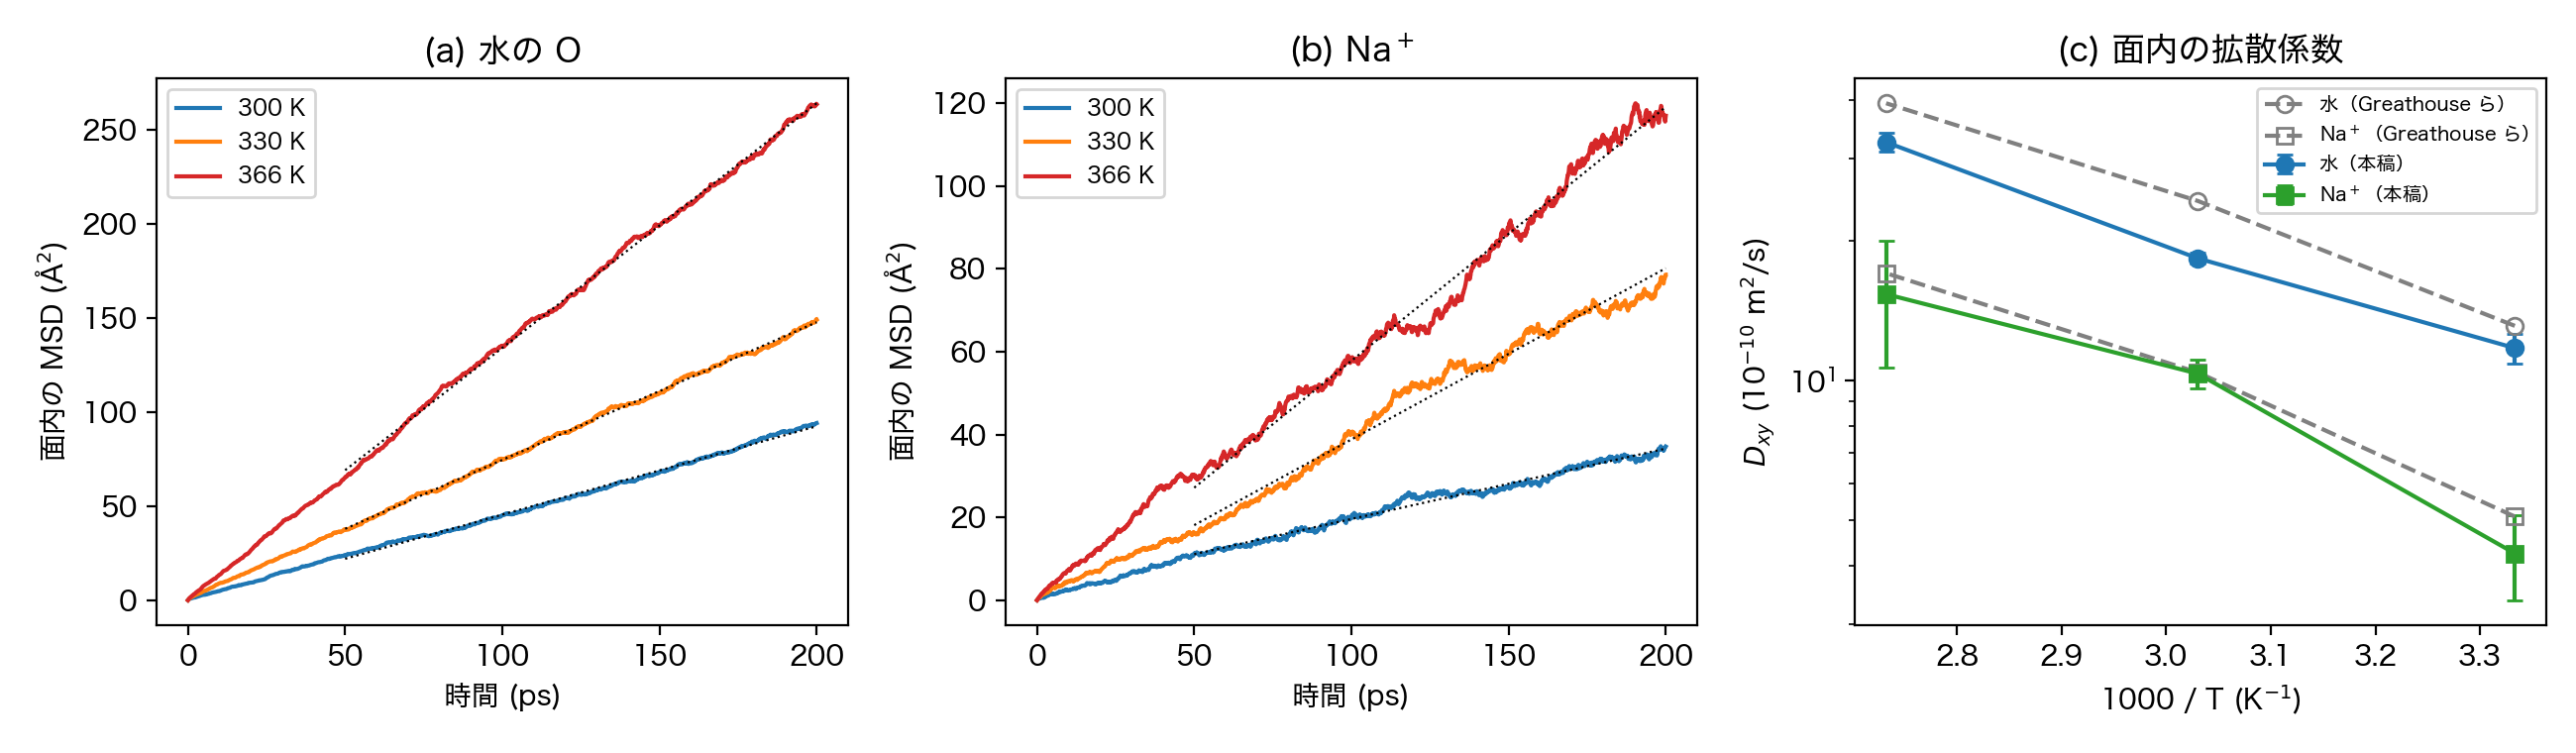
\includegraphics[width=\linewidth]{figs/diffusion.png}
\caption{Na モンモリロナイトの 2 水和層の層間の水の O と Na$^+$ の面内の拡散係数の温度依存性．本稿（構造ファイルから作った力場，4 区間の平均と標準誤差）と Greathouse ら\cite{greathouse2016}（ClayFF と柔軟な SPC 水，高電荷モデル）．}
\label{fig:diffusion}
\end{figure}

\subsection{白雲母の弾性定数と力学試験}
\label{sec:resmusc}
\paragraph{0\,K の弾性定数．}
応力 0 の箱は，入力の構造から a，b，c が $-0.5$，$-0.3$，$-1.5$\,\%，$\beta$ が $+0.4^\circ$ 違った．
弾性定数を表\ref{tab:musc}と図\ref{fig:musc}(a)に示す．
面内の $C_{11}$，$C_{22}$，$C_{66}$ は 264，235，95\,GPa で，実験（181，178，72\,GPa）より 46，32，32\,\% 大きく，Teich-McGoldrick らの ClayFF の値（236，198，94\,GPa）と同じく面内を大きく出した．
層に垂直な $C_{33}$（66.4\,GPa）は実験（58.6\,GPa）より 13\,\% 大きく，Teich-McGoldrick ら（67.6\,GPa）とよく一致した．
$C_{13}$，$C_{23}$（23.8，22.0\,GPa）は実験（25.6，21.2\,GPa）に近い．
一方，層をまたぐせん断の $C_{44}$，$C_{55}$（8.3，16.8\,GPa）は実験（16.5，19.5\,GPa）より 50，14\,\% 小さかった．
Teich-McGoldrick らの $C_{44}$ は $15.4\pm12.2$\,GPa と不確かさが大きい．
コンプライアンスから求めたヤング率は $E_x=234$，$E_y=213$，$E_z=62$\,GPa（Teich-McGoldrick ら 222，178，56.2\,GPa，実験 149，161，53.4\,GPa），せん断弾性率は $G_{yz}=8.3$，$G_{xz}=16.1$，$G_{xy}=95.2$\,GPa（実験 16.1，18.1，70.4\,GPa），体積弾性率（Reuss）は 54.2\,GPa（実験 48.7\,GPa）だった．
\paragraph{300\,K の引張とせん断．}
応力--ひずみ曲線を図\ref{fig:musc}(b)，(c)に示す（初期の応力はどれも 0.04\,GPa 以内）．
ひずみ 0.02 までの傾きから求めたヤング率は $E_x=224$，$E_y=222$，$E_z=58$\,GPa，せん断弾性率は $G_{xy}=90$，$G_{xz}=11.9$，$G_{yz}=9.2$\,GPa で，0\,K の値とおおむね合った．
Teich-McGoldrick らの 298\,K の値（218，190，69.4，83.9，19.6，15.2\,GPa）に対し，$E_x$ と $G_{xy}$ は 3，7\,\%，$E_y$ は 17\,\% 大きく，$E_z$ は 17\,\%，$G_{xz}$，$G_{yz}$ は 39\,\% 小さかった．
実験（149，161，53.5，70.4，18.1，16.1\,GPa）と比べると，面内の $E_x$，$E_y$，$G_{xy}$ は 28--50\,\% 大きく，層に垂直な $E_z$ は 8\,\% 大きく，層をまたぐ $G_{xz}$，$G_{yz}$ は 34--43\,\% 小さかった．
ポアソン比は $\nu_{yx}=0.42$，$\nu_{zx}=0.25$，$\nu_{xy}=0.36$，$\nu_{zy}=0.18$，$\nu_{xz}=0.07$，$\nu_{yz}=0.09$ で，Teich-McGoldrick ら（0.377，0.200，0.339，0.238，0.064，0.081）と同じく，面内の向き同士が大きく，層に垂直な向きへの応答が小さかった．
同じ構造ファイルから別の計算機（4 並列，ひずみ 0.10 まで）で回した計算でも，$E_x=221$，$E_y=219$，$G_{xy}=91$\,GPa で，3\,\% 以内で一致した．

引張は，どの向きも破断した．
強度（応力の最大値）は x で 14.7\,GPa（ひずみ 0.096），y で 13.4\,GPa（0.074），z で 3.5\,GPa（0.097），破断ひずみは x，y，z で 0.102，0.079，0.103 だった．
DelRio らの MD（25\,$^\circ$C）の破断応力（x，y で約 12\,GPa，z で約 3\,GPa）と破断ひずみ（x で約 9--10\,\%，y で約 7\,\%，z で約 10--11\,\%），Teich-McGoldrick らの破断ひずみ（x で約 0.095，y で約 0.075）と一致し，面内の強度が層に垂直な向きの約 4 倍という関係も同じだった．
せん断は，xy で 11.9\,GPa（ひずみ 0.147），xz で 2.9\,GPa（0.135），yz で 2.2\,GPa（0.127）が最大で，ひずみ 0.153，0.136，0.135 で破断した．
層の中の xy のせん断応力は，層をまたぐ xz，yz の 4--5 倍で，Teich-McGoldrick らの図 8（ひずみ 0.1 まで，約 4 倍）と同じ傾向だった．

\begin{table}[!htbp]
\centering
\caption{白雲母 2M$_1$ の弾性定数と弾性率（GPa）．本稿は構造ファイルから soapff-gui で作った力場（ClayFF，672 原子）．0\,K は静的な方法（ひずみ $\pm0.005$）の弾性定数とそのコンプライアンスから，300\,K は応力--ひずみ曲線の傾き（ひずみ 0.02 まで）から．Teich-McGoldrick ら\cite{teich2012}は ClayFF（5{,}376 原子）の表 1（0\,K）と表 2（298\,K）．実験は Vaughan と Guggenheim\cite{vaughan1986}のブリルアン散乱の値と，それから求めた弾性率．}
\label{tab:musc}
\small
\begin{tabular}{lrrrrr}
\toprule
 & \multicolumn{2}{c}{本稿} & \multicolumn{2}{c}{文献\cite{teich2012}} & 実験\cite{vaughan1986} \\
 & 0\,K & 300\,K & 0\,K & 298\,K & \\
\midrule
$C_{11}$ & 264.2 & & 236 & & 181.0 \\
$C_{22}$ & 235.3 & & 198 & & 178.4 \\
$C_{33}$ & 66.4 & & 67.6 & & 58.6 \\
$C_{44}$ & 8.3 & & 15.4 & & 16.5 \\
$C_{55}$ & 16.8 & & 14.1 & & 19.5 \\
$C_{66}$ & 95.3 & & 94.3 & & 72.0 \\
$C_{12}$ & 68.6 & & 41.9 & & 48.8 \\
$C_{13}$ & 23.8 & & 24.6 & & 25.6 \\
$C_{23}$ & 22.0 & & 40.0 & & 21.2 \\
\midrule
$E_x$ & 234 & 224 & 222 & 218 & 149 \\
$E_y$ & 213 & 222 & 178 & 190 & 161 \\
$E_z$ & 62.1 & 57.6 & 56.2 & 69.4 & 53.5 \\
$G_{yz}$ & 8.3 & 9.2 & 15.2 & 15.2 & 16.1 \\
$G_{xz}$ & 16.1 & 11.9 & 12.6 & 19.6 & 18.1 \\
$G_{xy}$ & 95.2 & 90.2 & 94.3 & 83.9 & 70.4 \\
\bottomrule
\end{tabular}
\end{table}

\begin{figure}[!htbp]
\centering
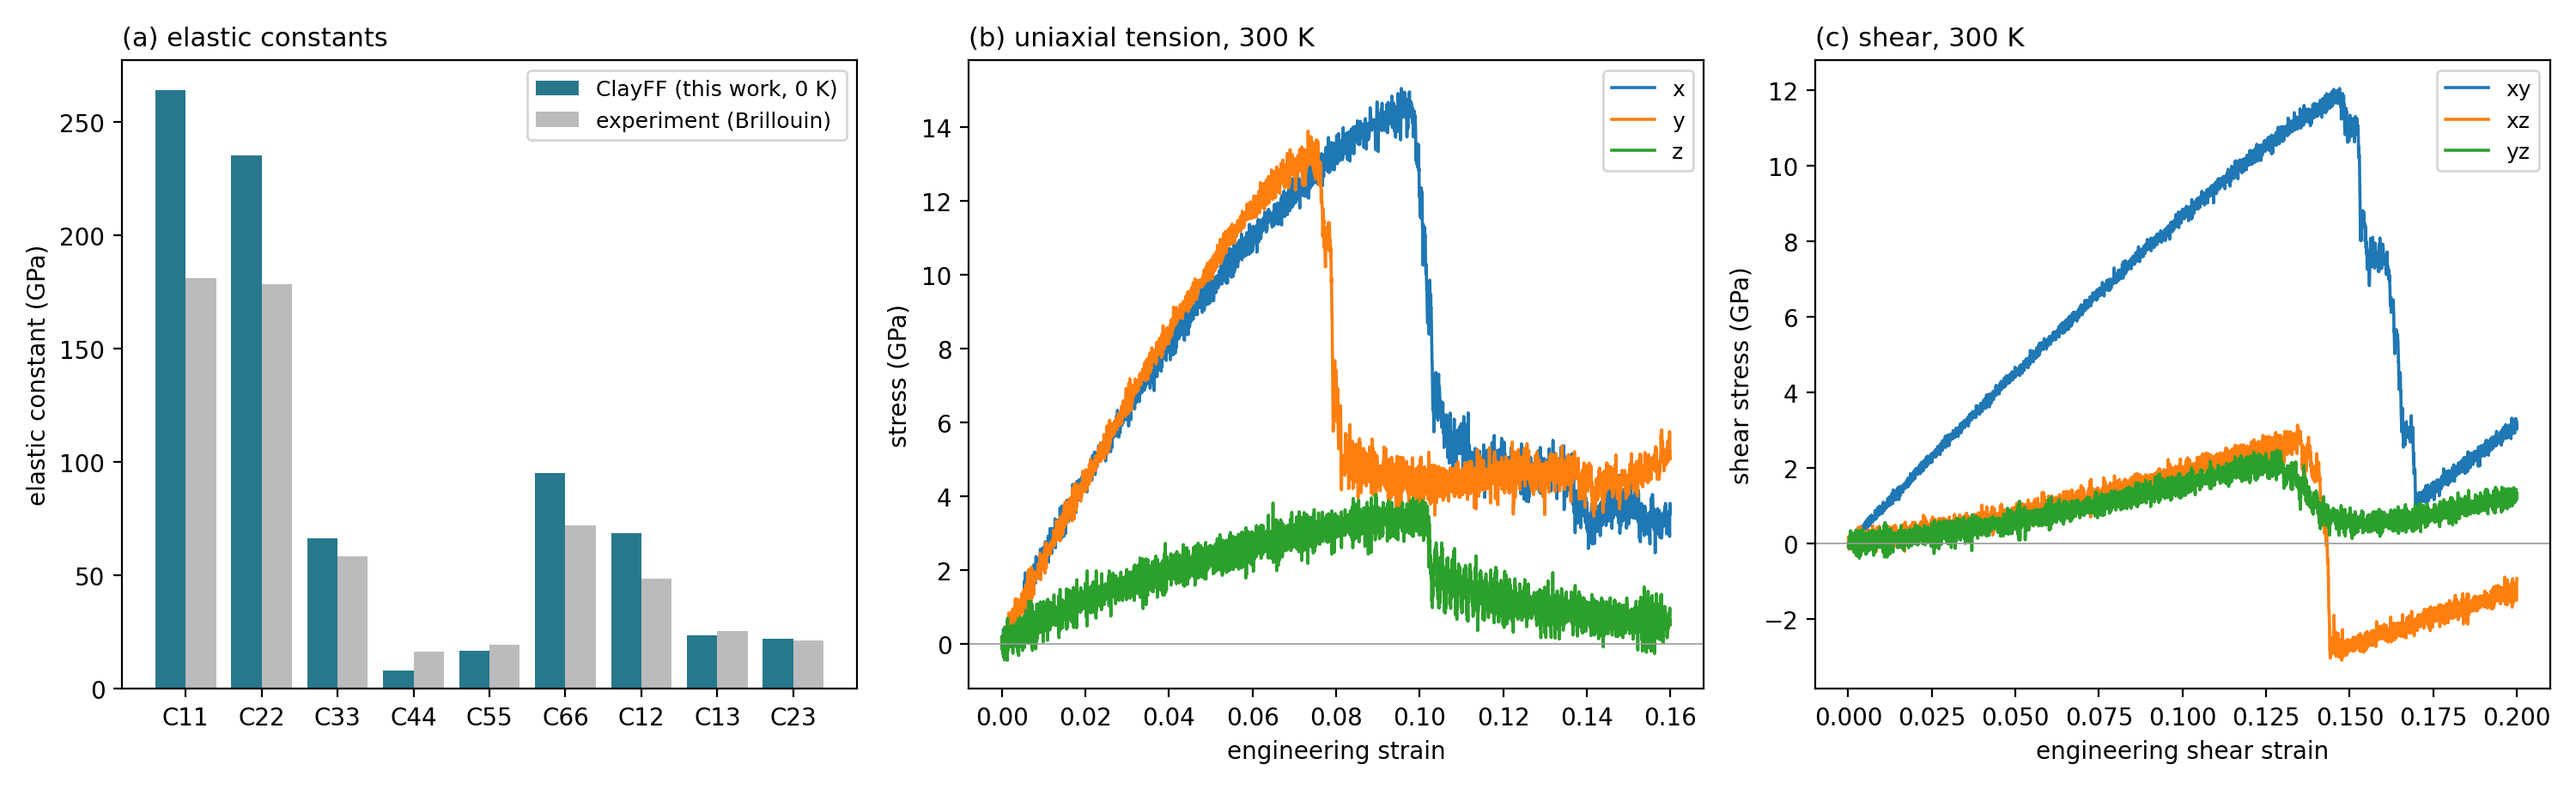
\includegraphics[width=\linewidth]{figs/muscovite.png}
\caption{白雲母 2M$_1$ の力学物性（構造ファイルから soapff-gui で作った力場）．(a) 0\,K の弾性定数と実験（ブリルアン散乱\cite{vaughan1986}）．(b) 300\,K の x，y，z の一軸引張（ひずみ速度 $10^9$\,s$^{-1}$，横の 2 方向は 1\,atm）．(c) 300\,K の xy，xz，yz のせん断．(b)，(c) は soapff-gui の「＋ 物性」で生成した入力を別の計算機で回したもの．}
\label{fig:musc}
\end{figure}

\section{計算できる鉱物と構造}
本稿で確かめた範囲，すなわち soapff-gui で現在計算できる鉱物と構造を表\ref{tab:scope}にまとめる．
ライブラリは Na モンモリロナイトと 12 の鉱物のバルクの結晶による 13 構造（5{,}878 原子）である．

\begin{table}[!htbp]
\centering
\caption{soapff-gui で計算できる鉱物と構造（本稿で確かめたもの）．}
\label{tab:scope}
\small
\begin{tabular}{p{2.6cm}p{6.4cm}p{5.2cm}}
\toprule
鉱物 & 構造 & 確かめたこと \\
\midrule
Na モンモリロナイト & Mg 置換の 2:1 層 2 枚と，層間の Na$^+$ と水 2 層（2 水和層），2{,}502 原子 & 全原子で型と電荷がライブラリと一致．水が粘土に重なった構造でも可．拡散係数を先行研究と比較 \\
石英 & バルクの結晶（SiO$_2$），162--216 原子 & 全原子で型と電荷が正解と一致 \\
アルバイト & バルクの結晶（NaAlSi$_3$O$_8$，Si--O--Al(IV) の O は obts），208--312 原子 & 同上 \\
ブルーサイト & バルクの結晶（Mg(OH)$_2$），240--500 原子 & 同上 \\
パイロフィライト & バルクの結晶（Al$_2$Si$_4$O$_{10}$(OH)$_2$，2 つの出典），320--720 原子 & 同上 \\
白雲母（2M$_1$，1M） & バルクの結晶（KAl$_2$(AlSi$_3$)O$_{10}$(OH)$_2$），168--672 原子 & 全原子で型と電荷が正解と一致．300\,K の MD のあとの構造でも一致．2M$_1$ の弾性定数と引張・せん断を実験・先行研究と比較 \\
金雲母 1M & バルクの結晶（KMg$_3$(AlSi$_3$)O$_{10}$(OH)$_2$），176--352 原子 & 全原子で型と電荷が正解と一致．MD のあとの構造でも一致（自分の参照が必要） \\
nanpingite & バルクの結晶（CsAl$_2$(AlSi$_3$)O$_{10}$(OH)$_2$），336--504 原子 & 同上（参照を除くと Cs は fallback） \\
カオリナイト，リザーダイト & 1:1 型の層のバルクの結晶，324--544 原子 & 全原子で型と電荷が正解と一致．MD のあとの構造でも一致 \\
タルク & バルクの結晶（Mg$_3$Si$_4$O$_{10}$(OH)$_2$），378--504 原子 & 同上 \\
\bottomrule
\end{tabular}
\end{table}

水のない結晶は，ライブラリの結晶と大きさの違う超格子でも，原子のまわりの環境が同じなので同じように扱える．
一方，次の構造は確かめておらず，ライブラリにその環境がないので扱えない．
\begin{itemize}
\item 結晶の表面と，鉱物と水の界面（切れた結合を水酸基で終端した表面を含む）．
\item 粘土のエッジ．
\item ほかの面，ほかの層間陽イオン（K$^+$，Cs$^+$，Ca$^{2+}$）や水の量の違うモンモリロナイト，置換の位置や層の数が違う構造（雲母の層間の K$^+$ と Cs$^+$ は確かめた）．
\item ほかの鉱物と，ClayFF に型のない元素（Ti，S など）や，ClayFF の型で中性にならない元素（Fe$^{2+}$ を含む annite など）を含む鉱物．
\end{itemize}
こうした構造を渡しても力場は作られるが，類似度が 0.95 未満の原子は ClayFF の型と電荷に戻され，0.95 以上でもライブラリにない環境の可能性がある．
出力される原子ごとの類似度と，分子と電荷の整合性の確認の結果で確かめ，必要ならその系の構造をライブラリに加える．

\section{議論}
SOAP と電荷の一対一の対応は，粘土の原子だけでなく，水と Na$^+$ を含めた系全体でも，ClayFF の型で表せる 4 つの鉱物の結晶を加えたライブラリ全体でも成り立った．
ClayFF の型と電荷は原子のまわりの結合のつながりで決まり，SOAP はそのつながりを区別できるので，構造ファイルの各原子にいちばん似たライブラリの原子の電荷と型をそのまま与えるだけで，電荷，型，結合，角度，LJ パラメータのそろった LAMMPS 入力ができる．
回帰ではなく，いちばん似た原子の電荷をそのまま使うので，出力は必ず ClayFF の電荷のどれかになり，同じ型には同じ電荷が付き，全体の電荷も保たれる．
結合を型から決めることで，原子が重なった構造でも正しい分子ができた．
ライブラリより大きい超格子の結晶でも，300\,K の MD で乱れた層状ケイ酸塩の結晶でも，全原子で正しい型と電荷が付いた．
参照を 1 つ除いた試験では，同じ種類の層を持つ鉱物がライブラリに残っていれば正しく型付けされたが，金雲母の Al(IV) と三八面体の Mg に囲まれた O のように，ほかの参照にない環境の原子は，類似度が 0.95 以上でも似た別の型（obts の代わりに ob）を取り違えた．
これは，類似度のしきい値だけでは誤りを防げない場合があり，新しい種類の鉱物を扱うときはその参照をライブラリに加える必要があることを示す．
ただし，この結果は，結晶の内部の原子のまわりの環境がライブラリの結晶と同じであることによる．表面，界面，エッジなど，ライブラリにない環境の原子は，類似度が下がるか，似た別の型を取り違えるおそれがある．
そのため，対象とする構造の種類ごとに，その構造をライブラリに加え，ライブラリの中の一対一の確認を行う必要がある．

力場は，ClayFF の原論文の表のとおりの ClayFF と柔軟な SPC 水で，SOAP が決めるのは電荷と型だけである．
そのため，結果は ClayFF の関数形とパラメータに依存し，ClayFF の型で表せない原子（ClayFF に型のない元素など）には使えない．

生成した力場の妥当性は，Na モンモリロナイトの層間の水と Na$^+$ の拡散係数と，白雲母の弾性定数と力学試験で確かめた．
拡散係数は，同じ ClayFF と SPC 水による Greathouse ら\cite{greathouse2016}の値の 0.75--0.99 倍で，活性化エネルギーは誤差の範囲で一致した．
白雲母では，ClayFF による先行研究\cite{teich2012,delrio2026}と同じく，面内の弾性率は実験より 30--50\,\% 大きく，層に垂直な引張の弾性率は実験に近く，破断応力と破断ひずみは先行研究の MD と一致した．
層をまたぐせん断の弾性率（$C_{44}$，$G_{xz}$，$G_{yz}$）は実験より小さく出た（\ref{sec:resmusc} 節）．
これらの差は，系の組成と大きさ，平均の方法，電荷の配置などの違いの範囲であり，構造ファイルから自動で作った力場は，手で型を決めた ClayFF と同じ物性を与える．

本稿で確かめたのは，Na モンモリロナイトと 12 の鉱物の結晶である．
置換の位置や層の数，水の量が違う構造，エッジ，表面や界面は確かめていない．

\section{結論}
ClayFF の電荷と SOAP の一対一の対応が，Na モンモリロナイトの水と Na$^+$ を含む系全体と，石英，アルバイト，ブルーサイト，パイロフィライトの結晶で成り立つことを示し，その対応から ClayFF（原論文の表のとおりのパラメータと柔軟な SPC 水）の LAMMPS 入力を自動で作り，最小化，緩和，MD，解析まで行う GUI ソフトウェア soapff-gui を開発した．
雲母，カオリン，蛇紋石，タルクの層状ケイ酸塩を加えた 13 構造のライブラリ（5{,}878 原子）の全原子で SOAP と電荷が一対一に対応した．
Na モンモリロナイトの初期構造では，水が粘土に重なっていても，構造ファイルから全原子の電荷と型がライブラリと一致する力場が作られた．
ライブラリと大きさの違う 12 の結晶（216--720 原子）と，300\,K の MD のあとの層状ケイ酸塩の結晶でも，全原子の電荷と型が結合のつながりから決めた ClayFF の型と一致した．
生成した力場による Na モンモリロナイトの層間の水と Na$^+$ の拡散係数は，同じ ClayFF による先行研究の 0.75--0.99 倍で，活性化エネルギーは一致した．
白雲母の弾性定数と引張・せん断の応力--ひずみ曲線も，ClayFF による先行研究とおおむね一致した．
利用者は構造ファイルを用意するだけでよく，原子の型分けや結合，角度，LJ パラメータの入力を手で書く必要がない．soapff-gui では，構造ファイルを選んで実行を押すだけで，力場の作成から LAMMPS の実行，拡散係数と PDF・RDF の解析，OVITO での表示までを行える．
そのため，ClayFF や LAMMPS に不慣れな学生や初学者でも粘土鉱物の MD を簡単に始められる道具として，研究だけでなく教育用途での活用も期待される．

\begin{thebibliography}{99}
\bibitem{cygan2004} R. T. Cygan, J.-J. Liang, A. G. Kalinichev, J. Phys. Chem. B \textbf{108}, 1255 (2004).
\bibitem{cygan2021} R. T. Cygan, J. A. Greathouse, A. G. Kalinichev, J. Phys. Chem. C \textbf{125}, 17573 (2021).
\bibitem{pouvreau2017} M. Pouvreau, J. A. Greathouse, R. T. Cygan, A. G. Kalinichev, J. Phys. Chem. C \textbf{121}, 14757 (2017).
\bibitem{lammers2017} L. N. Lammers, I. C. Bourg, M. Okumura, K. Kolluri, G. Sposito, M. Machida, J. Colloid Interface Sci. \textbf{490}, 608 (2017).
\bibitem{heinz2013} H. Heinz, T.-J. Lin, R. K. Mishra, F. S. Emami, Langmuir \textbf{29}, 1754 (2013).
\bibitem{behler2007} J. Behler, M. Parrinello, Phys. Rev. Lett. \textbf{98}, 146401 (2007).
\bibitem{bartok2010} A. P. Bart\'ok, M. C. Payne, R. Kondor, G. Cs\'anyi, Phys. Rev. Lett. \textbf{104}, 136403 (2010).
\bibitem{bartok2013} A. P. Bart\'ok, R. Kondor, G. Cs\'anyi, Phys. Rev. B \textbf{87}, 184115 (2013).
\bibitem{willatt2019} M. J. Willatt, F. Musil, M. Ceriotti, J. Chem. Phys. \textbf{150}, 154110 (2019).
\bibitem{musil2021} F. Musil, A. Grisafi, A. P. Bart\'ok, C. Ortner, G. Cs\'anyi, M. Ceriotti, Chem. Rev. \textbf{121}, 9759 (2021).
\bibitem{langer2022} M. F. Langer, A. Goe{\ss}mann, M. Rupp, npj Comput. Mater. \textbf{8}, 41 (2022).
\bibitem{de2016} S. De, A. P. Bart\'ok, G. Cs\'anyi, M. Ceriotti, Phys. Chem. Chem. Phys. \textbf{18}, 13754 (2016).
\bibitem{kancharlapalli2021} S. Kancharlapalli, A. Gopalan, M. Haranczyk, R. Q. Snurr, J. Chem. Theory Comput. \textbf{17}, 3052 (2021).
\bibitem{raza2020} A. Raza, A. Sturluson, C. M. Simon, X. Fern, J. Phys. Chem. C \textbf{124}, 19070 (2020).
\bibitem{dscribe} L. Himanen ほか, Comput. Phys. Commun. \textbf{247}, 106949 (2020).
\bibitem{smithdang} D. E. Smith, L. X. Dang, J. Chem. Phys. \textbf{100}, 3757 (1994).
\bibitem{nose1984} S. Nos\'e, Mol. Phys. \textbf{52}, 255 (1984).
\bibitem{hoover1985} W. G. Hoover, Phys. Rev. A \textbf{31}, 1695 (1985).
\bibitem{lammps} A. P. Thompson ほか, Comput. Phys. Commun. \textbf{271}, 108171 (2022).
\bibitem{catti1995} M. Catti, G. Ferraris, S. Hull, A. Pavese, Phys. Chem. Miner. \textbf{22}, 200 (1995).
\bibitem{ase} A. Hjorth Larsen ほか, J. Phys.: Condens. Matter \textbf{29}, 273002 (2017).
\bibitem{cod} S. Gra\v{z}ulis ほか, Nucleic Acids Res. \textbf{40}, D420 (2012).
\bibitem{ovito} A. Stukowski, Modelling Simul. Mater. Sci. Eng. \textbf{18}, 015012 (2010).
\bibitem{greathouse2016} J. A. Greathouse, R. T. Cygan, J. T. Fredrich, G. R. Jerauld, J. Phys. Chem. C \textbf{120}, 1640 (2016).
\bibitem{sova} M. Shiga, H. Morita, sova-cui (sovapy), \url{https://github.com/MotokiShiga/sova-cui}．
\bibitem{koneshan1998} S. Koneshan, J. C. Rasaiah, R. M. Lynden-Bell, S. H. Lee, J. Phys. Chem. B \textbf{102}, 4193 (1998).
\bibitem{perdikatsis1981} B. Perdikatsis, H. Burzlaff, Z. Kristallogr. \textbf{156}, 177 (1981).
\bibitem{vaughan1986} M. T. Vaughan, S. Guggenheim, J. Geophys. Res. \textbf{91}, 4657 (1986).
\bibitem{teich2012} S. L. Teich-McGoldrick, J. A. Greathouse, R. T. Cygan, J. Phys. Chem. C \textbf{116}, 15099 (2012).
\bibitem{delrio2026} F. W. DelRio, E. D. Hintsala, B. T. Dankesreiter, S. J. Grutzik, W. M. Mook, P. G. Kotula, H. S. Senanayake, J. A. Greathouse, A. G. Ilgen, ACS Mater. Lett. \textbf{8}, 2178 (2026).
\end{thebibliography}

\end{document}
